\chapter{Recolecci\'on y an\'alisis del corpus ZOOM}
\label{sec:corpus}

Hay tres \'areas principales en las que los corpora se pueden utilizar en la investigaci\'on sobre generaci\'on de expresiones referenciales:
evaluaci\'on, dise\~no y metodolog\'ias para la recolecci\'on de corpus \'utiles para investigaci\'on y el an\'alisis y modelizaci\'on estad\'istica de datos de corpora.
El desaf\'io de recopilaci\'on de corpus, se centra en torno al equilibrio que se necesita
entre el control de los par\'ametros experimentales tanto como sea necesario
y mantener la configuraci\'on de lo m\'as natural posible. 

Para evaluar la salida de un sistema, se puede 
comparar con los datos de corpora, bajo la premisa de que el objetivo de la comparaci\'on es
para evaluar si el sistema podr\'ia tener un modelo adecuado del comportamiento humano para la generaci\'on de expresiones referenciales.


El trabajo descripto en \cite{viethen} se encuadra en el \'area de an\'alisu y modelizaci\'on estad\'istica de datos de corpora. Entre otros resultados, este trabajo mostr\'o que, em lo que respecta a la GER, distintas personas pueden no  hacer lo mismo en la misma situaci\'on. De hecho, incluso la misma persona podr\'ia describir el mismo target de diferentes maneras en distintas ocasiones.
Este cap\'itulo se encuadra en las \'areas de dise\~no y metodolog\'ias para la recolecci\'on de corpus y su uso para evaluar sistemas de GER.
El corpus ZOOM es una colecci\'on de datos, resultante de un experimento realizado en un trabajo conjunto con la Universidad de S\~ao Paulo (Brasil). El objetivo del experimento fue crear un corpus de expresiones referenciales de un dominio m\'as complejo y m\'as cercano a las aplicaciones del mundo real, que los corpus existentes hasta el momento. Este corpus contiene referencias a targets singulares y plurales y hace gran uso de propiedades relacionales. Las descripciones del ZOOM corpus fueron producidas por humanos de espa\~nol y portugu\'es, lo cual permitir\'ia investigar la realizaci\'on ling\"u\'istica en estos lenguajes, que actualmente tiene pocos recursos. La mayor parte de los recursos del \'area est\'an en ingl\'es. Adem\'as permitir\'ia investigar la variaci\'on entre humanos en la GER (\cite{trainable-speaker,romina-coling,non-det}). 
En este Cap\'itulo se describe el dominio y las caracter\'isticas del corpus, la metodolog\'ia usada su recolecci\'on y anotaci\'on y se lo copara con trabajo previo. Luego haremos una evaluaci\'on en la Secci\'on~\ref{corpus-evaluacion} de los datos obtenidos. La evaluaci\'on realizada motiv\'o al caso de estudio de la Secci\'on \ref{sec:caso_estudio} en la que mostramos tres casos particulares de fragmentos de las ciudades de Lisboa y Madrid.

\section{Un corpus de descripciones de lugares en mapas de ciudades}

%\subsection{Caracter\'isticas del corpus}
%\label{corpus-caracteristicas}

%La recolecci\'on se llevo a cabo mediante una p\'agina web en la que registramos 20 ER dichas por cada persona. Cada persona di\'o 22 ER de mapas distintos, los primeros 2 mapas eran solamente para que la persona se acostumbre a usar el sistema, 11 de los cuales ten\'{i}an target singular, es decir s\'olo 1 target y los otros 11 target plural, es decir ten\'{i}an 2 targets.
En colaboraci\'on con el grupo de investigadores de procesamiento de lenguaje natural de la Universidad de S\~ao Paulo Brasil (EACH-USP) dise\~namos un experimento en la web para recolectar descripciones de ubicaciones en mapas. Las descripciones se recolectaron tanto en espa\~nol como en portugu\'es. El conjunto de datos obtenidos constituye un corpus de expresiones referenciales para investigaci\'on en GER y campos relacionados. Este trabajo se describe en \cite{DBLP:conf/acl/AltamiranoFPB15}.

Las situaciones de referencia en cuesti\'on hacen uso de mapas con dos grados de detalle (representados por los niveles de zoom), e incluyen descripciones singulares y plurales.



%.....................................
\subsection{Procedimiento de recolecci\'on del corpus}
%.....................................
\label{corpus-voluntarios}

Las ERs fueron hechas por personas voluntarias a las cuales se les envi\'o una invitaci\'on por correo electr\'onico o redes sociales. La parte en portugu\'es del corpus tuvo 93 participantes, siendo 66 (71\%) hombres y 27 (29\%) mujeres. El corpus espa\~nol tuvo 85 participantes, siendo 59 hombres (69\%) y 26 mujeres (30\%) como se muestra en la Figura \ref{estadistica-mf}.
\begin{figure}[ht]
\begin{center}
\frame{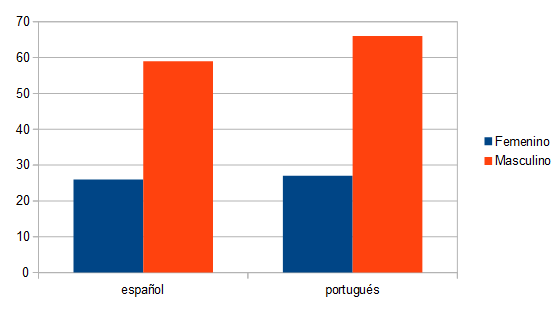
\includegraphics[width=10cm]{images/corpus/estadisticaFemMasc.png}}\\[0pt]
\caption{Estad\'istica de g\'enero de las personas que completaron el experimento.}
\label{estadistica-mf}
\end{center}
\end{figure}

Las personas voluntarias recibieron un link a la interfaz del experimento, como se muestra en la Figura~\ref{fig_pagPrincipal_seleccion_idioma}. Esa p\'agina conten\'{i}a las instrucciones para el experimento en 3 idiomas: ingl\'es, portugu\'es y espa\~{n}ol, y un link para completar el experimento en el idioma seleccionado. Las intrucciones solicitaban uma ER que permitiera a ``un amigo'' identificar puntos de inter\'es en mapas de ciudades. La idea es que la persona imaginara que estaba dando sugerencias a un amigo que posiblemente visitara dicha ciudad proximamente. 
\begin{figure}[ht]
\begin{center}
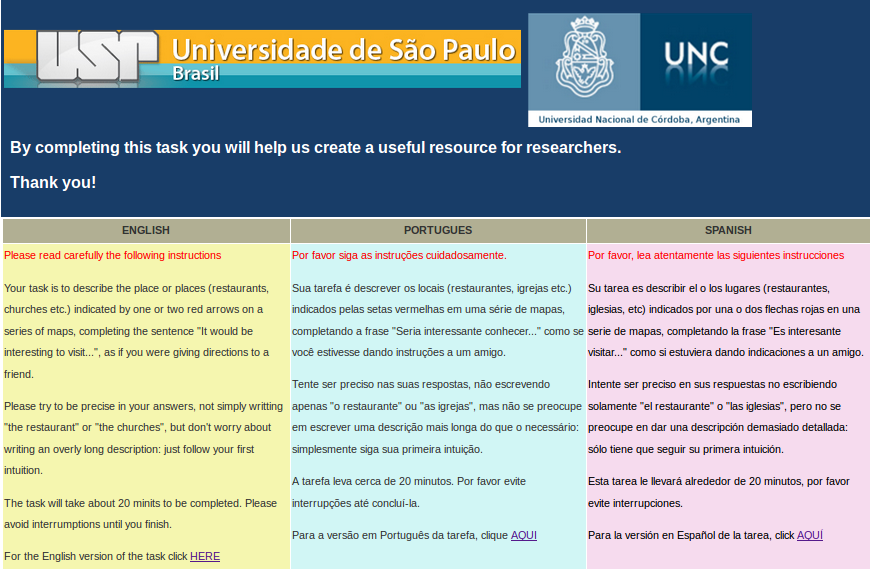
\includegraphics[width=17cm]{images/pagPrincipal.png}\\[0pt]
\caption{P\'agina principal del experimento.}
\label{fig_pagPrincipal_seleccion_idioma}
\end{center}
\end{figure}

\begin{figure}[H]
\begin{center}
\frame{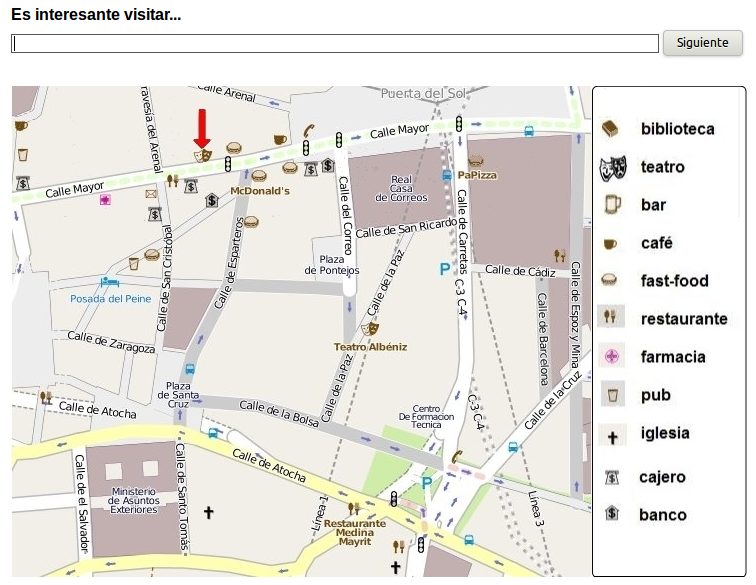
\includegraphics[width=17cm]{images/primerImagenRecortada.png}}\\[0pt]
\caption{Interface del experimento.}
\label{fig_interface}
\end{center}
\end{figure}

%Las instrucciones dec\'ian lo siguiente:\\
%``Su tarea es describir el o los lugares (restaurantes, iglesias, etc) indicados por una o dos flechas rojas en una serie de mapas, completando la frase; ``Es interesante visitar...'' como si estuviera dando indicaciones a un amigo. Intente ser preciso en sus respuestas no escribiendo solamente ``el restaurante'' o ``las iglesias'', pero no se preocupe en dar una descripci\'on demasiado detallada: s\'olo tiene que seguir su primera intuici\'on''

Lo que se pretend\'ia con esas instrucciones era por un lado que la persona d\'e una expresi\'on referencial del objeto o los objetos se\~nalados que sea un sintagma nominal, que dicha expresi\'on fuera natural como le dar\'ia a un amigo y por otro lado, no incentivar a la gente a hacer ER ni minimales ni sobreespecificadas, es decir, conseguir una expresi\'on natural. 
El experimento ped\'ia completar la frase ``Es interesante visitar...'' porque a dicha frase le falta un sintagma nominal para ser una oraci\'on gramaticalmente completa. Como las ER se realizan como sintagmas nominales, esa fue la construcci\'on gramatical generada por casi todas las personas que completaron el experimento.

Luego de seleccionar el idioma se mostraba la siguiente p\'agina, que recolectaba informaci\'on demogr\'afica, luego se mostraban los t\'erminos y condiciones\footnote{%
   \emph{ ``Acepto que los datos ingresados en este cuestionario sean usados an\'onimamente para investigaci\'on''.}
  }. 
Si la persona completaba los datos y aceptaba los t\'erminos y condiciones, se comenzaba el experimento mostrando, por ejemplo, el mapa de la Figura~\ref{fig_interface}.
La p\'agina ten\'{i}a una barra indicadora de progreso, la cual se iba actualizando a medida que el usuario completaba las ERs. Los mapas fueron mostrados en forma aleatoria y al final del experimento se mostraba un mensaje de agradecimiento.
Cada mapa mostraba un lugar determinado a ser descripto (por ejemplo, un restaurante, pub, teatro, etc.) se\~nalado por una flecha roja como se ve en la Figura \ref{fig_interface}. En esta figura, el lugar se\~nalado por la flecha es un teatro. En el caso de los mapas est\'imulo de ERs plurales se usaban 2 flechas como se ve en la Figura \ref{mapa20-5}, donde los lugares se\~nalados por las flechas son restaurantes. Despu\'es de completar la expresi\'on, la persona deb\'ia pulsar el bot\'on \emph{Siguiente} y entonces se seleccionaba otro est\'{i}mulo al azar y as\'{i} hasta el final del experimento. Las primeras 2 im\'agenes fueron mostradas s\'olo para que los participantes se familiarizaran con el entorno del experimento y las respuestas dadas no fueron guardadas.

\begin{figure}[H]
\begin{center}
\frame{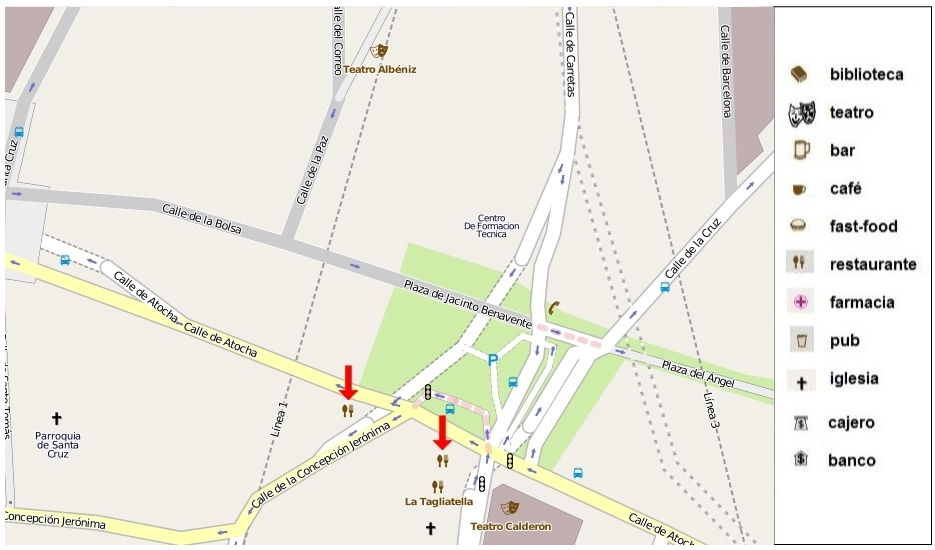
\includegraphics[width=15cm]{images/corpus/mapa20.png}}
\caption{Imagen del corpus ZOOM}
\label{mapa20-5}
\end{center}
\end{figure}
%\hspace*{0cm}
%\begin{minipage}[b]{0.5\linewidth}
%\centering
%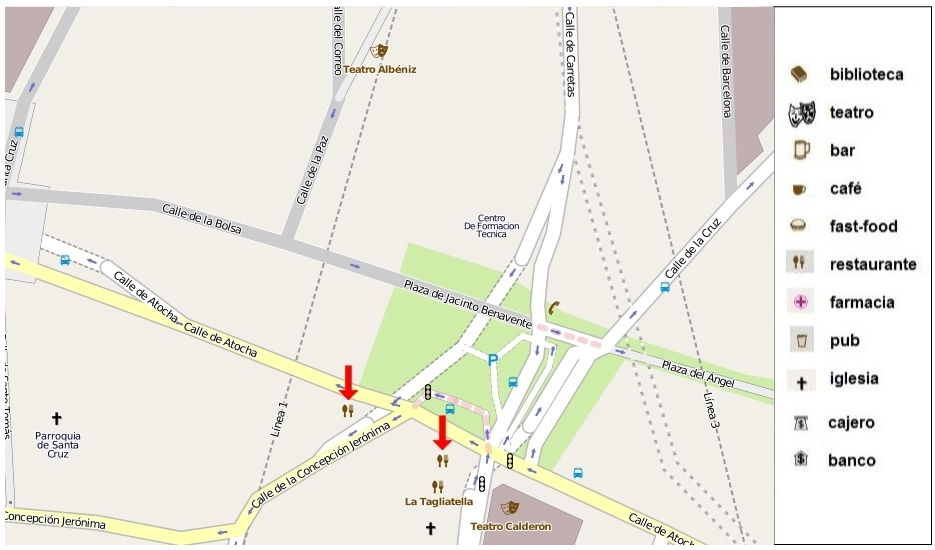
\includegraphics[width=\textwidth]{images/corpus/mapa20.png}%\\[0pt]
%\caption{Imagen del corpus ZOOM, con target plural.}
%\label{mapa20}
%\end{figure}




%.....................................
\subsection{Materiales utilizados en la recolecci\'on}
%.....................................
\label{corpus-materiales}

Para la recolecci\'on se usaron fragmentos de mapas de las ciudades de Lisboa y Madrid obtenidos desde openstreetmaps.org. Openstreetmaps.org es una p\'agina que tiene informaci\'on de mapas de todas partes del mundo, es una organizaci\'on en la que muchas personas de distintas partes del mundo colaboran para mantener la informaci\'on actualizada. Esta informaci\'on es de libre uso, es decir uno puede usar los mapas y s\'olo hay que nombrar de donde fueron sacados.
Se consideraron 2 idiomas: espa\~nol y portugu\'es. Se obtuvieron ERs para targets singulares como se v\'e por ejemplo en la Figura~\ref{fig_interface} y para targets plurales como se v\'e en la Figura~\ref{mapa20-5}. En los est\'imulos plurales se usaron referencias del mismo tipo (2 restaurantes, 2 iglesias, etc.) y adem\'as se tuvo en cuenta mapas con 2 niveles de zoom. El mapa de la Figura \ref{mapa20-5} muestra un fragmento del mapa de la Figura \ref{fig_interface} con un mayor nivel de zoom. Como se puede ver en las figuras, los mapas con mayor zoom (a las que describimos como zoom 2X) cubren una porci\'on m\'as chica de la ciudad pero, en general hay m\'as detalle.



%El experimento hizo uso de la p\'agina especialmente dise\~nada la cual se muestra en la Figura~\ref{fig-interface}. En esa p\'agina se observa el texto ``Es interesante visitar...'', abajo hay un espacio para que la persona ingrese la expresi\'on referencial, al lado esta el bot\'on ``Siguiente'' que  al presionarlo se guardaban los datos ingresados para el est\'imulo actual y se continuaba con el siguiente est\'imulo, de el lado derecho hab\'ia una barra de estado que mostraba el progreso hasta el momento, cada vez que se presionaba el bot\'on ``Siguiente'' la barra se actualizaba llen\'andose con color verde y mostrando el porcentaje que luego de 22 mapas llegaba al 100\%, debajo del indicador de progreso hab\'ia un link que dec\'ia ``Instrucciones'', el cual al pasar el cursor del mouse desplegaba las instrucciones mostradas al inicio.
%Del lado derecho del mapa se encontraba la leyenda, que mostraba para un conjunto de \'iconos del mapa que objetos significaban, se mostraron los siguientes (biblioteca, teatro, bar, caf\'e, fast-food, restaurante, farmacia, pub, iglesia, cajero, banco), esto se realiz\'o a fin de evitar confusi\'on a las personas que daban las expresiones referenciales, ya que se not\'o por ejemplo que los \'iconos de cajero y banco podr\'ian llegar a ser identificados como la misma palabra para distintas personas. 

Cada mapa conten\'ia \'iconos de lugares o cosas, calles, nombres de lugares, por ejemplo podemos ver en el mapa de la Figura~\ref{fig_interface} la Calle Mayor, ah\'i se pueden ver cajeros, restaurantes, fast-foods, caf\'e, tel\'efonos, correos, farmacias, sem\'aforos. Notar que algunos \'iconos tienen nombre, por ejemplo el fast-food McDonald's. Algunos edificios o plazas tambi\'en tienen nombre como la Real Casa de Correos y la Plaza de Pontejos. En el mapa tambi\'en podemos ver algunos objetos sin nombre.
Se puede ver en la Figura~\ref{fig_interface} el nombre del restaurante Medina Mayrit, pero en la Figura~\ref{mapa20-5} no se muestra el nombre, se v\'e s\'olamente el \'icono. Para el Teatro Alveniz se v\'e el nombre en ambos niveles de zoom. Notar que no siempre en el nivel 2X de zoom se ver\'a todo lo que se v\'e y m\'as que en el nivel X, como es el caso del restaurante Medina Mayrit, cuyo nombre se v\'e en la Figura~\ref{fig_interface} pero no se v\'e en la Figura~\ref{mapa20-5}.

Los mapas eran fragmentos del centro de la ciudad de Madrid (para la parte espa\~nola del corpus) y de Lisboa (para la parte portuguesa).
Para cada ciudad, se utilizaron 10 mapas con distintas ubicaciones. Cada ubicaci\'on se muestra con un nivel X y 2X de zoom, haciendo 20 im\'agenes en total. 
A diferencia de lo que se muestra en esta secci\'on a fines ilustrativos, en el experimento, en ambos niveles de zoom el objetivo se\~{n}alado se mantuvo. Algunos nombres de las calles y de landmarks pod\'{i}an no aparecer en diferentes niveles de zoom.
La mitad de las im\'agenes mostraron una sola flecha que apuntaba a un objeto en el mapa. Es decir, requer\'{i}an una descripci\'on como por ejemplo en la Figura~\ref{fig_interface} {\it el teatro que est\'a en la calle Mayor, cerca de un Macdonald's}. Mientras que la otra mitad mostraron dos flechas que apuntaban a dos lugares diferentes. Y por lo tanto requer\'ian una ER plural, como en Figura~\ref{mapa20-5} {\it los dos restaurantes sobre calle de Atocha cerca del Teatro Calder\'on}.


\subsection{Caracter\'isticas de los datos recolectados}
\label{sec:datos_recolectados}

La p\'agina web del experimento se mantuvo en l\'{i}nea hasta que se obtuvieron 100 experimentos completos para la parte en portugu\'es del corpus y 85  para la parte en espa\~nol. Luego de la verificaci\'on manual, se descartaron 602 descripciones portuguesas mal formadas y 366 descripciones espa\~nolas. As\'{i}, la parte portuguesa del corpus consta de 1.358 descripciones mientras que la parte espa\~nola contiene 1.234 ERs. 
Las descripciones mal formadas fueron descartadas siguiendo los siguientes criterios. A pesar de que las personas ten\'{i}an que completar la frase ``Es interesante visitar ...'' con un sintagma nominal que describe la ubicaci\'on se\~nalada por la flecha (o las flechas, en los casos plurales), algunas de las expresiones no eran frases nominales, sino frases completas, por ejemplo, \emph{``Vamos a ir a pizza express, es realmente barato''}, \emph{``No me gusta la comida r\'apida''}. Dichas frases fueron descartadas por no ser sintagmas nominales. Del mismo modo, se eliminaron todas las expresiones que describen un objeto que no sea el target previsto, las que utilizaban propiedades que no eran ciertas para el target, y las situaciones en que la persona ten\'{i}a que describir dos objetos pero describ\'ian s\'olo uno.La p\'agina fue dise\~nada para obtener el corpus en 3 idiomas (espa\~nol, portugu\'es e ingl\'es). Hasta el momento de escribir esta tesis se recolect\'o en dos idiomas: espa\~nol y portugu\'es. La p\'agina sigue en l\'inea, y el c\'odigo de la misma est\'a disponible para recolectar un corpus similar\footnote{http://cs.famaf.unc.edu.ar/~romina/pagina/}.

%En la Secci\'on~\ref{sec-problemas} se describen los criterios por los que se consideraron las descripciones mal formada.\textcolor{blue}{de esto ya hable antes...} Tambi\'en se discuten el desaf\'{i}o que supone obtener las ER en lenguaje natural en un experimento basado en la web para un dominio que es significativamente m\'as cerca de aplicaciones del mundo real que los corpus GER existentes.
En la parte portuguesa de los datos, el 78,6\% de las descripciones incluyen propiedades relacionales. Adem\'as de eso, el 36,4\% eran minimales un 44,3\% eran sobreespecificadas, y el 19,3\% eran subespecificadas. En la parte espa\~nola, 70\% de las descripciones incluyeron propiedades relacionales. Por otra parte, el 35\% eran minimales, el 40\% eran sobreespecificadas, y el 25\% eran subespecificadas.
Esta proporci\'on tan grande de descripciones subespecificadas as\'{i} como descripciones relacionales no son comunes en corpora de GER existente (o por lo menos en tal proporci\'on), esto puede reflejar la complejidad del dominio o limitaciones en el entorno web en el cual se bas\'o la obtenci\'on del corpus. Esto se discute en la Secci\'on \ref{corpus-anotacion}.



\subsection{Anotaci\'on del corpus}
\label{corpus-anotacion}

\begin{figure}[H]
\centering
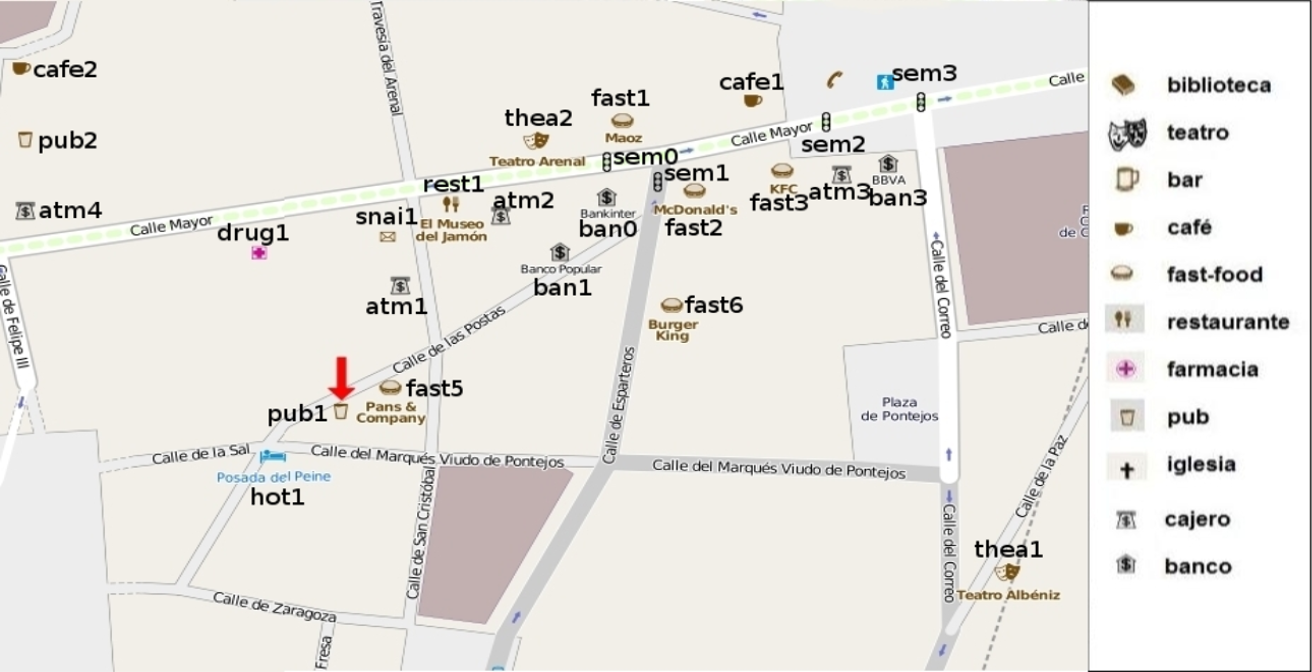
\includegraphics[width=\textwidth]{figures/ids.png}\\[0pt]
\caption{Mapa con Id's usado para la anotaci\'on.}
\label{mapa-con-ids}
\end{figure}

\begin{table}[H]
{\footnotesize
\begin{center}
\begin{tabular}{|l|l|r|r|r|}
\hline
N\'umero&Tipo & Nombre propio & En calle & ID\\
\hline

1&cafe & & & cafe2 \\
2&pub	& & & pub2 \\
3&atm	& & str1 & atm4 \\
4&drugstore & & str1 & drug1\\
5&snailpost & & str1,str2 & snai1\\
6&restaurant & el museo del jamon & str1,str2 & rest1\\
7&atm	& & str1 & atm2\\
8&theater & & str1 & thea2\\
9&semaphore & & str1 & sem0\\
10&semaphore & & str1 & sem1\\
11&semaphore & & str1 & sem2\\
12&semaphore & & str1,str3 & sem3\\
13&fast-food & maoz & str1 & fast1\\
14&fast-food & mcdonalds & str1,str4 & fast2\\
15&fast-food & kfc & str1 & fast3\\
16&cafe & & str1 & cafe1\\
17&fast-food & burger king & str4 & fast6\\
18&atm	& & str1 & atm3\\
19&pub	& & str1,str3 & ban3\\
20&fast-food & pans and company & str2 & fast5\\
\textbf{21}&\textbf{pub}	& & \textbf{str15} & \textbf{pub1}\\
22&hotel & posada del peine & str15,str19 & hot1\\
23&bank & banco popular & str15 & ban1\\
24&semaphore & & str1,str5 & rest5\\
25&fast-food & papizza & str5 & fast4\\
26&restaurant	& & str6,str7 & rest5\\
27&theater	& & str8 & thea1\\
28&semaphore & & str9 & sem5\\
29&semaphore & & str9 & sem6\\
30&restaurant & & str9 & rest2\\
31&church	& & str9,str10 & chur1\\
32&restaurant & medina mayrit & str9 & rest3\\
33&restaurant & & str9 & rest4\\
34&church & & str11 & chur2\\
35&bank & bankinter & str15 & ban0\\
36&street & calle mayor & & str1 \\
37&street & calle de san cristobal & & str2\\
38&street & calle del correo & & str3\\
39&street & calle de esparteros & & str4\\
40&street & calle de carretas & & str5\\
41&street & calle de espoz y mina & & str6\\
42&street & calle de cadiz & & str7\\
43&street & calle de la paz & & str8\\
44&street & calle de antocha & & str9\\
45&street & calle de santo tomas & & str10\\
46&street & calle de la cruz & & str11\\
47&street & calle del salvador & & str12\\
48&street & calle de la bolsa & & str13\\
49&street & calle de zaragoza & & str14\\
50&street & calle de las postas & & str15\\
51&street & calle botoneras & & str16\\
52&street & calle de gerona & & str17\\
53&street & calle de la sal & & str18\\
54&street & calle del marquez viudo de pontejos & & str19\\
\hline
\end{tabular}
\caption{Objetos identificados de la Figura~\ref{mapa-con-ids} indicando su tipo, su nombre propio (en caso de estar visible), calle (o calles) en las que se encuentra y un identificador \'unico. El target se resalta en negrita.\label{tabla-ids}}
%\vspace*{-.5cm}
\end{center}
%\end{small}
}
\end{table}

Para cada mapa se gener\'o una tabla con los identificadores \'unicos de los objetos visibles. Por ejemplo, para la imagen de la Figura~\ref{mapa-con-ids}, la tabla correspondiente es la Tabla~\ref{tabla-ids}. Los IDs se generaron usando las 3 o 4 primeras letras del tipo y un n\'umero correlativo dentro de ese tipo. Por ejemplo {\it pub1} es el que est\'a siendo apuntado por la fecha roja en la Figura~\ref{mapa-con-ids}, o sea es el target. A cada calle visible en el mapa tambi\'en se le asign\'o un identificador \'unico, como se ve en la Tabla~\ref{tabla-ids} desde la posici\'on  36. Dicha tabla tiene 4 columnas para cada objeto. El tipo es la representaci\'on sem\'antica del sustantivo que describe al objeto, por ejemplo, restaurante, bar, street. El nombre es el nombre propio del objeto, si ten\'ia, (se mantuvieron en el idioma original, espa\~nol o portugu\'es). ``en'', conten\'ia la calle en la que estaba situado el objeto, pod\'ia estar vac\'io si no estaba en una calle. Y el id que  fue compuesto por las 3 o 4 primeras letras del tipo del objeto m\'as un n\'umero para identificarlo un\'ivocamente, por ejemplo para los restaurantes ``rest1'', ``rest2''.

%- Los valores de los atributos se anotaron en Ingl\'es (por ejemplo, restaurant, pub, street, etc.), pero los nombres propios (para calles, etc.) se mantuvieron en su forma original, tal cual se v\'e en el mapa (Espa\~{n}ol, Portugu\'es).

Se seleccion\'o un conjunto fijo de atributos para cada objeto, pero dando flexibilidad con un atributo llamado ``other'' que permit\'ia anotar otras cosas que hayan aparecido en la expresi\'on dada por la persona, que no estuviera en la lista fija. En esta manera de anotar, cada objeto tiene como m\'aximo 26 posibles atributos.

En el caso de las descripciones plurales, el conjunto de atributos se repite para cada objeto, por lo que el anotador pod\'{i}a utilizar hasta 52 atributos.

Los 26 o 52 atributos nombrados anteriormente estan formados por:
10 atributos que denotan caracter\'isticas del objeto target, o relaciones del target con otros objetos.
\begin{itemize}
  \item tipo como por ejemplo, restaurant
  \item nombre propio como por ejemplo, McDonalds
  \item en calle como por ejemplo si el target est\'a en la {\it Calle Mayor} esta relaci\'on binaria entre el target y la calle tendr\'ia el identificador str1
  \item izquierda como por ejemplo en la Figura \ref{mapa-con-ids} pub1 est\'a a la izquierda de de fast5. En este caso, si el target fuera fast5, estar\'ia relacionado con la relaci\'on izquierda con pub1
  \item derecha como por ejemplo, en la Figura \ref{mapa-con-ids} fast5 est\'a a la derecha de de pub1
  \item en esquina, esta es una relaci\'on ternaria, es decir entre 3 objetos, el target y 2 calles. Esta clase de relaciones se ha modelado como 2 relacioines binarias    
  \item cerca como por ejemplo pub1 esta cerca de fast5
  \item en-frente-de como por ejemplo atm2 est\'a al frente de thea2
  \item detr\'as como por ejemplo detr\'as atm2 est\'a detr\'as de ban1
  \item otro cualquier otra cosa mencionada en la descripci\'on, pod\'ia ser una propiedad o relaci\'on. Por ejemplo un color. El atm2 azul
\end{itemize}
y 16 atributos que denotan los objetos adicionales (landmarks) que se mencionaron en la descripci\'on, a los cuales llamamos d1..d4. Por ejemplo, en {\it El pub que est\'a al lado de Pans \& Company, en la calle de las Postas}) tenemos:target = pub, d1 = fast-food (Pans \& Company) y d2 = Street (calle de las Postas).

Para cada target se consider\'o un m\'aximo 4 objetos tomados como puntos de referencia (landmarks), ya que con esta cantidad cubr\'iamos las descripciones m\'as largas, estos landmarks se anotaron como d1..d4, para cada landmark se anotaron 4 atributos:
\begin{itemize}
  \item Identificaci\'on (Id)
  \item Tipo (un sustantivo, restaurant, pub...)
  \item Nombre (Posada del Peine)
  \item Otro (alguna otra cosa dicha sobre el objeto)
\end{itemize}

A su vez cada atributo tiene una lista estricta de los valores permitidos. Por ejemplo, para el atributo tipo los posibles valores son biblioteca, teatro, bar, caf\'e, fast-food, etc. Tambi\'en se permite el valor ``otro'' que le d\'a al anotador una oportunidad de dar una respuesta cuando la descripci\'on muestra algo muy inusual.

Para los atributos espaciales (izquierda, cerca, etc.) permitimos que incluyan la mayor\'{i}a de los objetos en el mapa, a excepci\'on de aquellos que son claramente falsos. Por ejemplo, en el caso del atributo ``izquierda'' sus posibles valores incluyen la mayor\'{i}a de los objetos en el mapa de la Figura~\ref{mapa-con-ids}, a excepci\'on de los de la derecha del objeto target. Por ejemplo, es posible decir {\it el pub que esta a la izquierda de Pans \& Company}, pero no es admitido {\it el pub que est\'a a la izquierda de Posada del Peine}.




Las descripciones recolectadas fueron anotadas por dos anotadores independientes. Luego, un tercer anotador asumi\'o el rol de juez y di\'o la anotaci\'on final. El acuerdo entre los jueces, se midi\'o con el coheficiente Kappa \cite{kappa}, \'este fue del 84\% en el nivel de atributo.
Ambos, el contexto y las ERs se representaron en formato XML utilizando una versi\'on adaptada del formato XML adoptado en el corpus TUNA \cite{tuna-corpus}. Las ERs se agruparon en nodos TRIAL, que como se muestra en la Figura~\ref{xml}, que contienen informaci\'on general sobre cada persona (es decir, identificaci\'on, edad y sexo), seguido de su lista de respuestas. Cada respuesta identifica el contexto en que se produjo, y la ER que la persona dijo.
Al igual que en \cite{tuna-corpus}, el contenido de las ERs est\'an representadas por nodos que son conjunto de atributos que contienen una lista de nombres de atributos y sus valores. La Figura~\ref{xml} ilustra la representaci\'on para la ER {\it el pub que est\'a al lado de Pans \& Company, en la
calle de las Postas}.
\begin{figure}
%\tiny{
\begin{verbatim}
<TRIAL ID="2" SPEAKER="166" AGE="18" GENDER="m">
  <CONTEXT ID="3" SEQ="1300">
     <ATTRIBUTE-SET TARGET="pub1" LANDMARK="fast5" 
                    STRING="El pub que esta al lado de Pans & Company, 
                            en la calle de las Postas">
        <ATTRIBUTE NAME="type" VALUE="pub" />
        <ATTRIBUTE NAME="in" VALUE="str15" />
        <ATTRIBUTE NAME="landmark-name" VALUE="Pans & Company" />
     </ATTRIBUTE-SET>
  </CONTEXT>
</TRIAL>	
\end{verbatim}
%}
\caption{}\label{xml}
\end{figure}
%\normalsize


%In each description, attribute names for the first landmark object are preceded by the `landmark-' label as in the above example. Subsequent landmarks were labelled as `second-landmark' and so on. This was motivated by the need to provide unique attribute names for the benefit of GER algorithms.

%The set of images, text descriptions and their XML representations constitutes the Zoom corpus of referring expressions, to be made publicly available for research purposes. As a first step in this direction, the following sections present the results of a machine learning approach to GER based on the Portuguese portion of the data.

En cada TRIAL tenemos la informaci\'on de la identificaci\'on del TRIAL, de la persona, edad y g\'enero. En ATTRIBUTE-SET se encuentran los datos de la ER, TARGET y LANDMARKS con sus id's, STRING es la expresi\'on completa tal cual la di\'o la persona, y los atributos del target que en este ejemplo son su tipo pub, y su ubicaci\'on en la calle str15, en este caso hubo 1 s\'olo landmark. En casos donde hab\'ia m\'as de 1 landmark, los landmarks siguientes fueron etiquetados como ``second-landmark'' y as\'{i} sucesivamente. Esto fue motivado por la necesidad de proporcionar nombres de atributos \'unicos para el beneficio de los algoritmos de GER.
El conjunto de mapas, textos descriptivos y sus representaciones XML constituye el corpus ZOOM de ERs, el cual es p\'ublico para fines de investigaci\'on.  En lo que sigue presentamos una comparaci\'on de este corpus con corpora de ERs existentes hasta el momento. 

\subsection{Comparaci\'on con trabajo previo}
\label{sec:comparacion_trabajo_previo}

En la Tabla~\ref{tab-comparison} se presenta una comparaci\'on entre el corpus ZOOM y otros corpus de ERs existentes descripto en el Cap\'itulo~\ref{sec:seleccion}. La informaci\'on de dominio representa el n\'umero de posibles atributos at\'omicos m\'as el n\'umero de relaciones en cada descripci\'on (columna Atributos). La informaci\'on sobre el TUNA-corpus y las descripciones de ZOOM se basan s\'olo en la parte singular de cada corpus. La cantidad m\'axima de landmarks permitidos (en columna Landmarks). Tambi\'en se representa el tama\~no medio de la descripci\'on, es decir en n\'umero de propiedades anotadas, (en la columna tama\~no promedio). La columna Uso representa la utilizaci\'on de las propiedades, la cual se toma como la proporci\'on de las propiedades que aparecen en la descripci\'on sobre el n\'umero total de posibles atributos y puntos de referencia. Desde una perspectiva de GER, las ERs de mayor largo y las puntuaciones m\'as bajas de uso representan las situaciones m\'as complejas de referencia. Estas dos caracter\'isticas combinadas muestran que el corpus ZOOM es el m\'as complejo disponible en el \'area.


\begin{table}[H]
\begin{center}
\footnotesize{

\begin{tabular} {  l c c c c}
\hline
%\multicolumn{1}{c}{}
%&\multicolumn{1}{c}{Domain}
%&\multicolumn{3}{c}{Descriptions}\\
Corpus											& Atributos			& Landmarks			& Tama\~{n}o promedio	& Uso \\
\hline
TUNA-Furniture							& 4								& 0							& 3.1				& 0.8   \\
TUNA-People									& 10							& 0							& 3.1				& 0.3   \\
GRE3D3											& 9								& 1							& 3.4				& 0.3   \\
GRE3D7											& 6								& 1							& 3.0				& 0.4   \\
Stars												& 8								& 2							& 4.4				& 0.4   \\
Stars2											& 9								& 2							& 3.3				& 0.3   \\
Zoom-Pt											& 19							& 4							& 6.7				& 0.3   \\
Zoom-Sp											& 19							& 4							& 7.2				& 0.3   \\
\hline
\end{tabular}
}
\end{center}
\caption{Comparaci\'on con corpora de ERs existentes.}
\label{tab-comparison}
\end{table}



%2.3
%Craft
%The Craft corpus in Mitchell et al. (2010) addresses rather naturalistic situations
%of reference through face-to-face data collection involving craft objects (e.g.,
%feathers, beads, ribbons etc.). The focus of the data collection was mainly on
%the use of object-part relations, size comparisons and analogies. A group of 18
%subjects was requested to describe how to assemble four objects representing
%human faces by making use of pieces selected from a set of 51 craft objects. This
%resulted in a set of 505 references to single objects.
%2.4
%GenX
%The work in FitzGerald et al. (2013) addresses the issue of how to learn dis-
%tributions over logical forms for REG, and presents a corpus of descriptions
%of photographs of simple objects (e.g., cubes, cylinders etc.) called GenX. The
%GenX corpus was collected through crowd sourcing in monologue mode, and it
%does not contain relational descriptions.
%The corpus is largely devoted to reference to sets (including both situations of
%plurality and coordination) but it does include a subset of singular descriptions
%(846 instances). GenX descriptions were produced in 269 situations of reference
%and were semi-automatically labelled with three identifying attributes (type,
%colour and shape) including instances of negation (e.g., 'the red toy that is not
%a
%
%

%%.....................................
%\subsection{Discusi\'on}
%%.....................................
%\label{corpus-discusion}

%Previous corpora of referring expressions have been collected in specially designed and highly controlled domains. Collecting corpora from a domain that is directly relevant to real-world applications poses a significant challenge not only to the collection and annotation process itself but also to existing GER algorithms. This is made evident by the large proportion of referring expressions that needed to be manually discarded from our dataset because the did not constitute a referring expression of the intended target. This proportion is 30\% for the Portuguese portion of the dataset and 23\% for the Spanish portion. 

%The ill-formed descriptions were discarded following the criteria that we explain here. As seen in Figura~\ref{fig-interface} subjects had to complete the sentence ``It would be interesting to visit ...'' with a noun phrase describing the location signalled by the arrow. However, some of the referring expressions were not noun phrases but full sentences. For example, responses such as ``Let's go to pizza express, it's really cheap'' were discarded because the subject had in mind a communicative goal other than identifying the target. Moreover, a few subjects completed the experiment with sentences like ``I don't like fast food'' which were clearly out of domain. Similarly, we removed all expressions that described an object other than the intended target, which used properties that were not true of the target, all situations in which the subject had to describe two objects but described only one, and all descriptions containing only the basic attribute type (as in ``the church'').

%After this cleaning process the Portuguese portion of the corpus still contains a 19.3\% of underspecified referring expressions and the Spanish portion a 25\%. An example of underspecified referring expression is shown in Figura~\ref{fig-interface}; the referring expression ``the pub at Cowgate'' is underspecified because there are two pubs at Cowgate street on the map. The percentage of underspecified referring expressions in the Zoom corpus is much higher than that reported in the corpora described in the the previous section, which is not higher than 5\%. Previous psycholinguistic studies~\cite{Clark1986} have found that over 20\% of the referring expressions in naturally occurring discourse are underspecified with respect to the established context. In sufficiently complex domains,~\cite{Clark1986} found that speakers will often produce an initial underspecified referring expression, and then repair it if necessary instead of producing a uniquely identifying description from the start. As discussed in 
%the previous section, the Zoom domain is likely contain more complex situations of reference if compared to existing resources of this kind, that is,  Zoom description are on average longer, and have a lower average attribute usage. This, in our opinion, may explain the high proportion of referential underspecification in our data.   

%The proportion of overspecified referring expressions of the Zoom corpus is similar to that found in previous work. However, the proportion of relational descriptions is presently higher. Relational descriptions constitute a challenge for GER algorithms due to the computational complexity associated to their generation~\cite{survey}. A further challenge posed by the Zoom corpus is the fact that it contains two descriptions for every target based on different - but related - models corresponding to the same map location seen with different zoom levels. For instance a map with higher zoom level (2X) is illustrated in Figura~\ref{fig-with-zoom}, and the same map with lower zoom level is shown in Figura~\ref{fig-interface}. 


Los corpora de expresiones referenciales existentes se caracterizan por su dise\~no y recolecci\'on en experimentos muy controlados. La reco sino tambi\'en para pilaci\'on de corpus de un dominio que es directamente relevante para aplicaciones del mundo real plantea un reto importante no s\'olo para los algoritmos de GER existentesel proceso de recolecci\'on y anotaci\'on en s\'{i}. Esto se hace evidente por la gran proporci\'on de las expresiones referenciales que deben ser desechadas desde nuestra base de datos porque no constituyen una ER para el objeto target. Esta proporci\'on es del 30\% de la parte portuguesa del corpus y el 23\% de la parte espa\~nola del corpus.
Despu\'es de este proceso de limpieza, la parte portuguesa del corpus contiene todav\'{i}a un 19,3\% de expresiones referenciales subespecificadas y la parte espa\~nola un 25\%. El porcentaje de ERs subespecificadas en el corpus ZOOM es mucho mayor que lo reportado en los corpora de ERs descriptos en el la Secci\'on~\ref{sec:corpus2}, que no es mayor que el 5\%. 

Estudios psicoling\"u\'{i}sticos~\cite{Clark1986} han encontrado que m\'as del 20\% de las ERs son subespecificadas con respecto al contexto establecido. En dominios relativamente complejos, se encontr\'o que los hablantes a menudo producen una ER subespecificada inicial, y luego agregan m\'as informaci\'on si es necesario, en lugar de producir una descripci\'on que identifica al target de forma un\'{i}voca desde el principio. El dominio del ZOOM corpus es probable que contenga situaciones m\'as complejas de referencia que los corpora existentes de este tipo. Es decir, las descripciones del ZOOM son en promedio m\'as largas, y tienen un promedio de uso de atributos dio m\'as bajo. Esto en nuestra opini\'on, puede explicar la alta proporci\'on de subespecificaci\'on en nuestros datos. La proporci\'on de descripciones relacionales tambi\'es es mayor que en el trabajo anterior. Las descripciones relacionales constituyen un desaf\'{i}o para los algoritmos de GER debido a la complejidad computacional asociada a su generaci\'on~\cite{survey}. Otro desaf\'{i}o que plantea el corpus ZOOM es el hecho de que contiene dos descripciones para cada objeto target bas\'andose en diferentes modelos correspondientes a la misma ubicaci\'on en el mapa visto con diferentes niveles de zoom. 
\begin{figure}[ht]
\begin{center}
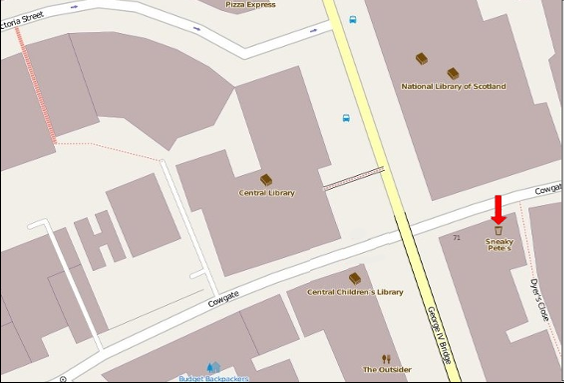
\includegraphics[width=8.5cm]{images/interface2-b.png}\\[0pt]
\caption{Mapa con nivel de zoom X.}
\label{interface2}
\end{center}
\end{figure}
Por ejemplo, un mapa con mayor nivel de zoom (2X) se ilustra en la Figura~\ref{fig-with-zoom}, y el mismo mapa con un menor nivel de zoom se muestra en la Figura~\ref{interface2}.

\begin{figure}[H]
\begin{center}
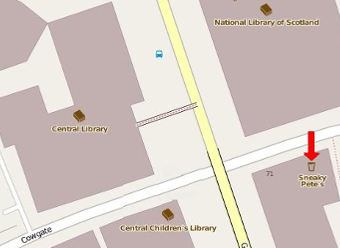
\includegraphics[width=8.5cm]{images/with-zoom.jpg}\\[0pt]
\caption{Mapa con nivel de zoom m\'as detallado (2X).}
\label{fig-with-zoom}
\end{center}
\end{figure}

%The underlying models for these two maps are different but not unrelated. The map with 2X zoom contains fewer objects but may include more properties due to the added level of detail. The  referring expression for the target in the 1X map may or may not be the same as in the 2X map. For instance, the referring expression  ``the pub at Cowgate'' is underspecified on the 1X map, but it is minimally distinguishing on the 2X map. Changes of this kind are common in interactive applications.  The context of reference during an interaction changes in structure, in the number of objects and referable properties. The challenge for GER algorithms would be to produced an appropriate description for the modified context without starting from scratch. GER algorithms based on local (rather than global) context partitioning (e.g.,~\cite{areces08}) seem to have an advantage in this respect, and in this sense we hope that the Zoom data will help the research in the field to move forward.

 Los modelos subyacentes de estos dos mapas son diferentes, pero esta\'an relacionados. El mapa con zoom 2X contiene menos elementos, pero con m\'as propiedades debido al mayor nivel de detalle. Una ER para el target en el mapa 1X puede o no ser \'util en el mapa 2X. Por ejemplo, la expresi\'on referencial ``el pub en Cowgate'' es subespecificada en el mapa 1X, pero es minimal en el mapa 2X. Cambios de este tipo son comunes en aplicaciones interactivas: cambios en la estructura del contexto de referencia durante una interacci\'on, en el n\'umero de objetos y en las propiedades a las cuales hay que referirse. El desaf\'{i}o para los algoritmos de GER ser\'{i}a producir una descripci\'on apropiada para el contexto modificado sin empezar desde cero. Estos temas se discuten en mayor detalle en el Cap\'itulo \ref{sec:conclusiones}. 

%%%%%%%%%%%%%%%%%%%%%%%%%%%%%%%%%%%%%%%%%%%%%%%%%%%%%%%%%%%%%%%%%%%%%%%%%%%%%%%%%%%%%%%%%%%%%%%%%%%%%%%%%%%%%%%%%%%%%%%%%%%%%%%%%%%%%%%%%%%%%%%%%%%%%%%%%%
\section{Desempe\~no de otros algoritmos sobre el corpus ZOOM}
%%%%%%%%%%%%%%%%%%%%%%%%%%%%%%%%%%%%%%%%%%%%%%%%%%%%%%%%%%%%%%%%%%%%%%%%%%%%%%%%%%%%%%%%%%%%%%%%%%%%%%%%%%%%%%%%%%%%%%%%%%%%%%%%%%%%%%%%%%%%%%%%%%%%%%%%%%
\label{corpus-evaluacion}
%\textcolor{blue}{decidir si esta parte la dejo o no, mas me gustaria poner evaluacion para la parte en espanol}

%In this section we illustrate the use of the Zoom corpus as training and test data for a machine learning approach to GER adapted from \cite{thiago-svm}. The  goal of this evaluation is to provide reference results for future comparison with purpose-built GER algorithms, and not to present a complete GER solution for this or other domains.
En esta secci\'on se presentan los resultados del desempe\~no de un algoritmo simb\'olico el algoritmo incremental descripto en la Secci\'on \ref{sec:algo_incremental} y un algoritmo puramente estad\'istico basado en support vector machines (SVM). Estos algoritmos se eval\'uan sobre un fragmento del corpus ZOOM para poner en perspectiva los resultados de nuestro algoritmo presentado en la Secci\'on \ref{sec:caso_estudio}.
%.....................
\subsection{Algoritmos y procedimiento}
%......................

%We used a subset of singular descriptions from the Portuguese portion of the corpus. This comprises  821 descriptions produced in 9 scenes. Evaluation was carried out by comparing the corpus description with the system output to measure overall accuracy (i.e., the number of exact matches between the two descriptions), Dice \cite{dice} and MASI \cite{masi} coefficients (i.e., the degree of overlap between the algorithm output and the corresponding corpus description).

%Following \cite{thiago-svm}, we built a GER model using support vector machines with radial basis function kernel. The classifiers were trained and tested using 6-fold cross validation. Optimal parameters were selected using grid search as follows:for each step in the main cross-fold validation, one fold is reserved for testing, and the remaining $k-1$ folders are subject  to a second cross-validation procedure in which different parameter combinations are attempted. The $C$ parameter is assigned the values 1, 10, 100 and 1000, and $\gamma$ is assigned 1, 0.1, 0.001 and 0.0001. The best-performing parameter set is selected to build a classifier trained from the $k-1$ folders, and tested on the test data. This procedure is repeated for every iteration of the main cross-validation procedure.

Para esta evaluaci\'on publicada en \cite{altamirano15} se utiliz\'o un subconjunto de descripciones singulares de la parte portuguesa del corpus. Esto comprende 821 descripciones producidas por personas para 9 escenas. La evaluaci\'on se llev\'o a cabo mediante la comparaci\'on de las ERs del corpus con la salida del sistema para medir la exactitud global (es decir, el n\'umero de coincidencias exactas entre las dos descripciones), los coeficientes Dice \cite{dice} y MASI \cite{masi} (es decir, el grado de solapamiento entre la salida del algoritmo y la descripci\'on corpus correspondiente).

El algoritmo SVM utilizado se basa en un dise\~no propuesto en \cite{thiago-svm}. Es decir se construye un modelo de GER usando {\it clasificadores support vector machines} (SVM) con funci\'on de kernel radial kernel de base radial. Los clasificadores se entrenaron y se hicieron validaciones cruzadas con {\it 6 folders}. Para conseguir los par\'ametros \'optimos se realiz\'o lo el procedimiento est\'andar de k-folders. Es decir, para cada validaci\'on cruzada, se reserv\'o un conjunto para las pruebas, y los restantes $k-1$ conjuntos quedaron sujetos a un segundo procedimiento de validaci\'on cruzada en el que se probaban diferentes combinaciones de par\'ametros. Al par\'ametro $C$ se le asignaron los valores 1, 10, 100 y 1000, y a $\gamma$ se le asignaron los valores 1, 0,1, 0,001 y 0,0001. El conjunto de par\'ametros de mejor desempe\~no fue seleccionado para construir un clasificador entrenado on los conjuntos $k-1$, y probado en los datos de prueba. Este procedimiento se repiti\'o para cada iteraci\'on del procedimiento principal de validaci\'on cruzada.
%................................
%\subsection{Modelo Computacional }
%................................

%The present model consists of 12 binary classifiers representing whether individual referential attributes should be selected for inclusion in an output description. The classifiers correspond to atomic attributes of the target and first landmark object ({\em type}, {\em name} and {\em others}), and relations. Referential attributes of other landmark objects were not modelled due to data sparsity and also to reduce computational costs. For similar reasons, the multivalue {\em between} relation is also presently disregarded, and `corner' relations involving two landmarks (e.g., two streets) will be modelled as two separate classification tasks.

%Two learning features were considered by each classifier:{\em landmarkCount}, which represents the number of landmark objects near the main target, and {\em DistractorCount}, which represents the number of objects of the same type as the target within the relevant context in the map.

%From the outcome of the 12 binary classifiers, a description is built by considering atomic target attributes in the first place. For every positive prediction, the corresponding atomic attribute is selected for inclusion in the output description. Next, relations are considered. If no relation is predicted, the algorithm terminates by returning an atomic description  of the main target object. If the description includes a relation, the related landmark object is selected  as well, and the algorithm is called recursively to describe the next object.

%Since every attribute that corresponds to a positive prediction is always selected, the algorithm does not regard uniqueness as a stop condition. As a result, the output description may convey a certain amount of overspecification.


El modelo SVM consta de 12 clasificadores binarios que representan si los atributos individuales deben ser seleccionados para su inclusi\'on en la ER de salida. Los clasificadores se corresponden con atributos at\'omicos del target y del primer landmark con los atributos ({\em tipo}, {\em nombre } y {\em otros}), y las relaciones. Los atributos de otros landmarks no se modelaron en este experimento. El valor m\'ultiple de la relaci\'on {\em entre} tambi\'en se ignor\'o, y la relaci\'on esquina que implica a dos puntos de referencia (por ejemplo, dos calles) se modelaron como dos tareas de clasificaci\'on independientes.

Dos caracter\'{i}sticas de aprendizaje fueron consideradas por cada clasificador: {\em landmarkCount}, que representa el n\'umero de objetos cercanos al target, y {\em DistractorCount}, que representa el n\'umero de objetos del mismo tipo que el target en el contexto considerado.

A partir de los resultados de los 12 clasificadores binarios, una descripci\'on se construy\'o teniendo en cuenta los atributos at\'omicos del target en primer lugar. Por cada predicci\'on positiva, se seleccion\'o el atributo at\'omico correspondiente para su inclusi\'on en la descripci\'on de salida. A continuaci\'on, se consideraron las relaciones. Si no se elije ninguna relaci\'on, el algoritmo termina devolviendo una descripci\'on at\'omica del objeto target. Si la descripci\'on incluye una relaci\'on, se selecciona el objeto landmark relacionado, y el algoritmo se llama de forma recursiva para describir a ese objeto.

Puesto que cada atributo que se corresponde con una predicci\'on positiva ser\'a siempre seleccionado, el algoritmo no considera unicidad como una condici\'on de parada. Como resultado, la descripci\'on de salida puede transmitir una cierta cantidad de sobreespecificaci\'on o bien ser subespecificada.


%......................
\subsection{Resultados de la generaci\'on }
%......................

%Table \ref{tab-reg-results} summarizes the results obtained by the GER algorithm built from SVM classifiers, those obtained by a baseline system representing a relational extension of the Dale \& Reiter Incremental Algorithm, and by a Random selection strategy.  
Tabla \ref{tab-reg-results} resume los resultados obtenidos por el algoritmo de GER construido a partir de clasificadores SVM, los obtenidos mediante un sistema descripto en el Cap\'itulo \ref{sec:seleccion} que implementa una extensi\'on relacional del algoritmo incremental \cite{incremental}, y por una estrategia de selecci\'on random. Se comparan precisi\'on, coeficientes Dice y MASI.

% these results are for SVM.All.VAR-   compared to the AEI- baseline
\begin{table}[H]
\begin{center}
\begin{tabular} {  l c c c }
\hline
{Algoritmo}							& {Precisi\'on} 	& { Dice}		& MASI \\ \hline 
SVM											& 0.15		& 0.51			& 0.28 \\
Incremental							& 0.04		& 0.53			& 0.21 \\
%Selecci\'on Random        	& 0.03    & 0.45      & 0.15 \\
\hline
\end{tabular}
\end{center}
\caption{Resultados de la GER.}
\label{tab-reg-results}

\end{table}

%In what follows we compare accuracy scores obtained by every algorithm pair using the chi-square test, and we compare {\em Dice} scores using {\em Wilcoxon's} signed-rank test.

%In terms of overall accuracy\footnote{And also in terms of MASI scores, although this is presently not further discussed.}, the SVM approach outperforms both alternatives. The difference from the second best-performing algorithm (i.e., the Incremental approach) is highly significant ($\chi^{2}=$ 79.87, df=1, p$<$0.0001). Only in terms of Dice scores an opposite effect is observed (T=137570.5, p$=$ 0.01413). 

%We also assessed the performance of the individual classifiers. Table \ref{tab-svm-results} shows these results as measured by precision (P), recall (R), F1-measure (F1) and area under the ROC curve (AUC). 


En lo que sigue se comparan los resultados de exactitud obtenidos por cada par algoritmos mediante la prueba de chi cuadrado, y se compara {\em Dice} utilizando la prueba de rangos con signo {\em de Wilcoxon}.

En t\'erminos de exactitud global y tambi\'en en cuanto a las puntuaciones MASI, el m\'etodo SVM supera al algoritmo incremental. La diferencia con el segundo algoritmo de mejor rendimiento (es decir, el enfoque incremental) es altamente significativa ($\chi^{2}=$ 79,87, df = 1, p$<$ 0,0001). S\'olo en cuanto a las puntuaciones de {\it Dice} se observa el efecto contrario (T = 137570.5, p$=$0,01413).

Tambi\'en se evalu\'o el desempe\~no de los clasificadores individuales. La Tabla \ref{tab-svm-results} muestra estos resultados, medida por la exactitud (P), exhaustividad (R), F1-medida (F1) y el \'area bajo la curva ROC (AUC).

%these are the rsults for the training over the set of ALL speakers 
\begin{table}[H]
\begin{center}
\footnotesize{

\begin{tabular}{l c c c c }
\hline
{{Clasificador}}	& {P} & {R} & {$F_{1}$} & {AUC} \\
\hline
{{tg\_type}} 			& 0.95 & 1.00 & 0.98 & 0.25 \\
{{tg\_name}}			& 0.09 & 0.05 & 0.07 & 0.41 \\
{{tg\_other}}			& 0.00 & 0.00 & 0.00 & 0.05 \\                               
{{lm\_type}}			& 0.93 & 1.00 & 0.96 & 0.44 \\                               
{{lm\_name}}			& 0.97 & 1.00 & 0.98 & 0.35 \\                               
{{lm\_other}}			& 0.00 & 0.00 & 0.00 & 0.43 \\                               
{{next-to}}				& 0.50 & 0.24 & 0.32 & 0.63 \\                               
{{right-of}}			& 0.00 & 0.00 & 0.00 & 0.28 \\                               
{{left-of}}				& 0.00 & 0.00 & 0.00 & 0.27 \\                               
{{in-front-of}}		& 0.00 & 0.00 & 0.00 & 0.42 \\                               
{{behind-of}}			& 0.00 & 0.00 & 0.00 & 0.17 \\                               
{{in/on/at}} 			& 0.60 & 0.60 & 0.60 & 0.61 \\                               
\hline                   
\end{tabular}
\caption{Resultados del clasificador a nivel atributo.}
\label{tab-svm-results}
}
\end{center}
\end{table}
\normalsize

%From these results we notice that highly frequent attributes (e.g., type and name) were classified  with high accuracy, whereas others (e.g., multivalue attributes and relations) were not. 

A partir de estos resultados se ve de que algunos atributos (por ejemplo, el tipo del target y del landmark y el nombre del landmark) se clasificaron con gran exactitud, mientras que otros (por ejemplo, las relaciones) no se clasificaron con alta precisi\'on.

Cabe destacar que aunque en estas m\'etricas, el algoritmo SVM supera al incremental, el SVM no puede asegurar que su salida sea una ER dado que no usa el modelo para verificar si la descripci\'on identifica un\'ivocamente al target, mientras que el algoritmo incremental s\'i. El algoritmo SVM podr\'ia verse entonces como una posible implementaci\'on de la fase ``generar'' del modelo cognitivo e Keysar \cite{keysar:Curr98} discutido en la Secci\'on \ref{sec:psicolinguistica}, a la que le falta la fase de ``ajustar'' para poder asegurar unicidad. Como tal genera ERs de una forma \textbf{egoc\'entrica} (en terminolog\'ia de Keysar et al) como lo har\'ia un ni\~no. Nuestro algoritmo en cambio, implementa las dos fases del modelo cognitivo de Keysar et al.

A continuaci\'on evaluamos el desempe\~no de nuestro algoritmo sobre mapas del corpus ZOOM.

\section{Desempe\~no de nuestro algoritmo sobre el corpus}
\label{sec:caso_estudio}

En esta secci\'on presentamos tres casos de estudio detallados de evaluaci\'on de las ERs generadas con nuestros algoritmos para mapas del corpus ZOOM. En la Secci\'on \ref{sec:sinzoom} analizaremos la generaci\'on de rankings de ERs singulares en el dominio del corpus ZOOM y compararemos el desempe\~no del algoritmo con datos del corpus. En la Secci\'on \ref{sec:conzoom} analizaremos la generaci\'on de rankings de ERs en un mapa con mayor nivel de zoom que el analizado en la Secci\'on \ref{sec:sinzoom}. En la Secci\'on \ref{sec:plural} analizaremos la generaci\'on de ERs plurales.

%  Veremos las diferencias entre esos mapas a nivel de informaci\'on disponible, obtendremos a partir de cada imagen el modelo subyacente que usar\'a el algoritmo y a partir de las ER's del corpus obtendremos las probabilidades de uso de las palabras, para luego ejecutar el algoritmo. Compararemos las ER's dadas por el algoritmo con las que dieron las personas.

%En cada uno de los mapas, el o los targets est\'an se\~nalados por flechas rojas, seg\'un la leyenda que se ubica a la derecha, podemos decir que si se trata de una iglesia, o restaurantes, etc. 
%
%\textcolor{blue}{
%Podria explicar un poco porque restringimos el modelo... a parte de lo que se ve en el mapa. paper Incremental generation of spacial referring expressions in situated dialog cuenta un poco como generar las ER de un robot en tiempo real, van acotando el entorno. Tambien hablan de las preferencias pero ponen nombres raros topologial constrstivem topological relative topological proyective contrastive proyective relative. (Bryant et al. 1992 Gapp 1995) above/below sobre in front of/behind y de esta sobre to the right of / to the left of
%}


\subsection{Generaci\'on de expresiones refenciales singulares}
\label{sec:sinzoom}

Consideremos el mapa de la Figura \ref{mapa-zoom1} que muestra una regi\'on de la ciudad de Madrid. El target, es decir, el objeto se\~nalado por la flecha roja, es una iglesia, como se puede ver en la leyenda ubicada a la derecha del mapa. En la parte inferior derecha de la imagen se muestran las probabilidades de uso, las cuales fueron aprendidas desde el corpus, como se describe en el Cap\'itulo \ref{sec:algoritmo}, estas probabilidades no estaban en la imagen mostrada a los participantes que completaron el experimento de recolecci\'on de corpus, se agregaron a la imagen para ilustrar la discusi\'on de esta secci\'on.

En la Tabla \ref{freq-mapa} se muestran las 10 expresiones referenciales m\'as frecuentes generadas por las personas que participaron 
en la recolecci\'on del corpus para el mapa de la Figura \ref{mapa-zoom1}. Se indica el porcentaje de personas que dieron cada tipo de ER, es decir la cantidad de distintas personas que independientemente decidieron usar la misma ER\footnote{Por la misma ER nos referimos a una ER con la misma sem\'antica. Posibles divergencias gramaticales o l\'exicas en la realizaci\'on fueron unificadas.} para referirse al target, dividido por la cantidad total de ERs del mapa (se d\'a en porcentaje). Estas 10 ERs m\'as frecuentes acumulan el 78.5\% del total de las ERs del corpus para el mapa considerado. Tambi\'en se indica sin son subespecificadas (SubE) o sobreespecificadas (SobreE). Notar que las que no son ni subespecificadas, ni sobreespecificadas, son minimales.\\


%\end{figure}
\begin{figure}
\begin{center}
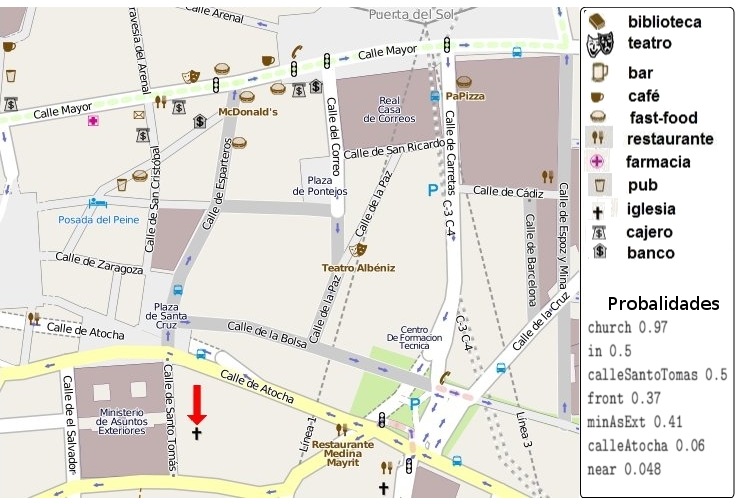
\includegraphics[width=\textwidth]{images/corpus/mapa6-prob.png}
\caption{Imagen del corpus ZOOM con target singular. Se muestran las probabilidades de uso de las palabras en la esquina inferior derecha.}
\label{mapa-zoom1}
\end{center}
\end{figure}

Para ejecutar el algoritmo necesitamos definir el vocabulario del modelo, es decir las palabras que vamos a usar al correr el algoritmo, la sem\'antica del mismo. Estas palabras fueron sacadas de la anotaci\'on del corpus, el cual est\'a anotado en ingl\'es.\\

%\DeclareFloatFont{tiny}{\tiny}% "scriptsize" is defined by floatrow, "tiny" not

%\begin{table}[H]
%{\footnotesize
%%\texttiny
%%\floatsetup[table]{font=tiny}
%\begin{center}
%\begin{tabular}{|l|l|c|c|c|c|}
%\hline
%&ER 					      & \# &  \% & SubE & SobreE\\ \hline \hline
%1&La iglesia 																																		 &16&19.7\%  & X & \\ \hline
%2&Iglesia en la calle de Santo Tom\'as																									 &15&18.5\% 	&  & \\ \hline
%3&Iglesia en la calle de Santo Tom\'as frente al Ministerio de Asuntos Exteriores        &11&13.6\% &  &X \\ \hline
%%&Asuntos Exteriores& &&&\\ \hline
%4&Iglesia frente al Ministerio de Asuntos Exteriores 													 &11&13\% &  & \\ \hline
%5&Iglesia en la calle Santo Tom\'as cerca del Ministerio de Asuntos Exteriores        &2 &2.5\% &  &X \\ \hline
%%&Asuntos Exteriores& & & & \\ \hline
%6&Iglesia en la calle de Atocha																									 &2&2.5\%  &  & \\ \hline
%7&En calle de Santo Tom\'as 																													 &2&2.5\% 	& X & \\ \hline
%8&Iglesia que est\'a en la calle de Santo Tom\'as y Atocha, frente al 									 &2&2.5\%	&  &X \\ 
%&Ministerio de Asuntos Exteriores																		 &&&& \\ \hline
%9&Iglesia que est\'a en la calle de Santo Tom\'as y Atocha										 &2&2.5\% 	&  &X \\ \hline
%10&Iglesia cerca del Ministerio de Asuntos Exteriores														 &1&1.2\% 	&  & \\ \hline
%\end{tabular}
%\caption{10 ER m\'as frecuentes del corpus para el mapa de la Figura \ref{mapa-zoom}.}\label{freq-mapa}
%\end{center}
%}%\end{tiny}
%\end{table}
\begin{table}[H]
{\footnotesize
%\texttiny
%\floatsetup[table]{font=tiny}
\begin{center}
\begin{tabular}{|l|l|c|c|c|}
\hline
&ERs del corpus ZOOM para el target \emph{church1} 					       &  \% & SubE & SobreE\\ \hline \hline
1&Iglesia 																																		 &19.7\%  & X & \\ \hline
2&Iglesia en la calle de Santo Tom\'as																									 &18.5\% 	&  & \\ \hline
3&Iglesia en la calle de Santo Tom\'as frente al Ministerio de Asuntos Exteriores        &13.6\% &  &X \\ \hline
%&Asuntos Exteriores& &&&\\ \hline
4&Iglesia frente al Ministerio de Asuntos Exteriores 													 &13\% &  & \\ \hline
5&Iglesia en la calle Santo Tom\'as cerca del Ministerio de Asuntos Exteriores        &2.5\% &  &X \\ \hline
%&Asuntos Exteriores& & & & \\ \hline
6&Iglesia en la calle de Atocha																									 &2.5\%  &  & \\ \hline
7&En calle de Santo Tom\'as 																													 &2.5\% 	& X & \\ \hline
8&Iglesia que est\'a en la calle de Santo Tom\'as y Atocha, frente al 									 &2.5\%	&  &X \\ 
&Ministerio de Asuntos Exteriores																		 &&& \\ \hline
9&Iglesia que est\'a en la calle de Santo Tom\'as y Atocha										 &2.5\% 	&  &X \\ \hline
10&Iglesia cerca del Ministerio de Asuntos Exteriores														 &1.2\% 	&  & \\ \hline
\end{tabular}
\caption{Las 10 ER m\'as frecuentes del corpus para el mapa de la Figura \ref{mapa-zoom1}.}\label{freq-mapa}
\end{center}
}%\end{tiny}
\end{table}

\vspace*{-0.5cm}

%Algunas personas dijeron ``en la esquina de...'', eso fue anotado como ``between'' y luego 2 calles, esta palabra no fue usada para correr el algoritmo porque tiene 2 par\'ametros, en cambio usamos ``in'' para ambas calles, con esa modificaci\'on, no estamos perdiendo informaci\'on ya que si el algoritmo da ambas calles, lo podr\'iamos realizar como ``esquina''. Se muestra el vocabulario y las probabilidades de uso de las palabras del vocabulario, sacadas del corpus, para el mapa de la Figura \ref{mapa-zoom}.

%\begin{table}[H]
%\begin{small}
%\begin{center}
%\begin{tabular}{|l|c|}
%\hline
%Palabra 					      &  Probabilidad\\ \hline \hline
%church & 0.97\\
%in & 0.5\\
%calleSantoTomas & 0.5\\
%front & 0.37\\
%minAsExt & 0.41\\
%calleAtocha & 0.06\\
%near & 0.048\\

%\hline
%\end{tabular}
%\caption{Probabilidad de las palabras del dominio.}\label{prob-vocabulario}
%\end{center}
%\end{small}
%\end{table}
Para calcular las probabilidades de uso usamos el m\'etodo presentado en el Cap\'itulo \ref{sec:algoritmo}, cuando se tiene un corpus disponible para la escena considerada. Se tuvieron en cuenta las ERs que dieron las personas, incluso las que eran subespecificadas, pero no las que no eran ciertas, un total de 63 ERs fueron las que cumpl\'ian con esas condiciones. Para cada palabra de las que aparec\'ia en el corpus para el contexto seleccionado, las cuales son: \{church, in, front, near, minAsExt, calleSantoTomas, calleAtocha\} se cont\'o la cantidad de veces que aparec\'ia la palabra en el corpus, teniendo en cuenta que si aparec\'ia 2 veces en la misma ER se contaba s\'olo 1 vez, a fin de tener siempre probabilidades entre 0 y 1, y luego se dividi\'o sobre 63 que fueron la cantidad de ERs que eran v\'alidas. Por ejemplo la palabra {\it church} apareci\'o en 61 ERs, por lo tanto la probabilidad de {\it church} es 61/63 = 0.968. Y as\'i se calcul\'o para las dem\'as palabras del vocabulario. Las probabilidades de uso de las palabras se muestran en la esquina inferior derecha del mapa de la Figura \ref{mapa-zoom1}.
En la Figura \ref{modelo-mapa-zoom} se muestra el modelo relacional que usamos como input del algoritmo. A fines ilustrativos, el modelo representa s\'olo la parte del mapa que est\'a al sur de la calle Atocha.

\begin{figure}[H]
\centering
\begin{tikzpicture}
  [
    n/.style={circle,draw,inner sep=5pt,node distance=4cm},
    aArrow/.style={scale=10,->, >=stealth, thick,
    shorten <= 1pt, shorten >= 1pt},
  ]
	\node[n,label=below:{
    \relsize{-2}$\begin{array}{c}
     \nStreet\end{array}$}] (a) {\relsize{-2}$str17$};		
			
	\node[n,label=below:{
    \relsize{-2}$\begin{array}{c}
      \nCalleDeElSalvador\end{array}$}, right of=a] (b) {\relsize{-2}$str12$};
  
	\node[n,label=below:{
    \relsize{-2}$\begin{array}{c}
      \nCalleDeLaCruz\end{array}$}, right of=b] (m) {\relsize{-2}$str16$};		 

\node[n,label=below:{
    \relsize{-2}$\begin{array}{c}
      \nCalleSantoTomas\end{array}$}, above of=b] (c) {\relsize{-2}$str10$};	
				
 \node[n,label=above:{
    \relsize{-2}$\begin{array}{c}
      \nBuilding\\[-3pt] 
      \nMinAsExt\end{array}$}, above of=a] (f) {\relsize{-2}$min1$};	
					
  \node[n,label=above:{
    \relsize{-2}$\begin{array}{c}
     \nChurch\end{array}$}, above of=f] (g) {\relsize{-2}$church1$};
			
 \node[n,label=above:{
    \relsize{-2}$\begin{array}{c}
     \nChurch\end{array}$}, right of=c] (d) {\relsize{-2}$church2$};
			
  \node[n,label=above:{
    \relsize{-2}$\begin{array}{c}
      \nRestaurante\\[-3pt] 
      \nMedinaMayrit\end{array}$}, above of=d] (h) {\relsize{-2}$rest3$};			
			
 \node[n,label=above:{
    \relsize{-2}$\begin{array}{c}
    \nCalleAtocha\end{array}$}, above of=c] (e) {\relsize{-2}$str9$};		

\node[n,label=below:{
    \relsize{-2}$\begin{array}{c}
    \nRestaurante\end{array}$}, right of=m] (k) {\relsize{-2}$rest4$};

\node[n,label=below:{
    \relsize{-2}}, right of=d] (i) {\relsize{-2}$d$};
		
 \node[n,label=above:{
    \relsize{-2}$\begin{array}{c}
    \nCalleDeCarretas\end{array}$}, above of=i] (j) {\relsize{-2}$str15$};	

%\node[n,label=below:$str17\nStreet$,label=above:{
 %   \relsize{-2}}, below of=k] (n) {};				
 \draw [aArrow,<->,bend right=40] (g) to node[auto,swap]{\relsize{-2}$\nFrenteCerca$} (f);
% \draw [aArrow,bend right=40] (f) to node[auto,swap]{\relsize{-3}$\nFrenteCerca$} (g);

 \draw [aArrow,bend right=40] (g) to node[auto,swap]{\relsize{-2}$\nIn$} (c);
 \draw [aArrow,bend right=20] (g) to node[auto,swap]{\relsize{-2}$\nIn$} (e);

 \draw [aArrow,bend right=40] (d) to node[auto,swap]{\relsize{-2}$\nIn$} (m);
 \draw [aArrow,<->,bend right=-10] (d) to node[auto,swap]{\relsize{-2}$\nFrenteCerca$} (i);
 %\draw [aArrow,bend right=40] (i) to node[auto,swap]{\relsize{-2}$\nFrente$} (d);
 \draw [aArrow,<->,bend right=40] (k) to node[auto,swap]{\relsize{-2}$\nCerca$} (d);
 %\draw [aArrow,bend right=40] (d) to node[auto,swap]{\relsize{-2}$\nCerca$} (k);
 \draw [aArrow,<->,bend right=80] (k) to node[auto,swap]{\relsize{-2}$\nCerca$} (h);

 \draw [aArrow,bend right=40] (k) to node[auto,swap]{\relsize{-2}$\nIn$} (m);
 \draw [aArrow,<->,bend right=20] (k) to node[auto,swap]{\relsize{-2}$\nFrenteCerca$} (i);
% \draw [aArrow,bend right=40] (i) to node[auto,swap]{\relsize{-2}$\nFrente$} (k);
 \draw [aArrow,bend right=20] (h) to node[auto,swap]{\relsize{-2}$\nIn$} (e);
 \draw [aArrow,bend right=-20] (h) to node[auto,swap]{\relsize{-2}$\nIn$} (j);

 \draw [aArrow,bend right=30] (f) to node[auto,swap]{\relsize{-2}$\nIn$} (c);
 \draw [aArrow,bend right=40] (f) to node[auto,swap]{\relsize{-2}$\nIn$} (e);
 \draw [aArrow,bend right=40] (f) to node[auto,swap]{\relsize{-2}$\nIn$} (a);
 \draw [aArrow,bend right=40] (f) to node[auto,swap]{\relsize{-2}$\nIn$} (b); 

 \draw [aArrow,bend right=5] (i) to node[auto,swap]{\relsize{-2}$\nIn$} (e);
 \draw [aArrow,bend right=40] (i) to node[auto,swap]{\relsize{-2}$\nIn$} (m);
%\draw[dotted] (-0.5,-1.1) rectangle (10.5,3.1);

 \end{tikzpicture}
\caption{Modelo relacional del mapa de la Figura \ref{mapa-zoom1}.}
\label{modelo-mapa-zoom}
\end{figure}
La iglesia target se representa como {\it church1} y la iglesia distractora como {\it church2}. La iglesia target se encuentra {\it near} y {\it front} a el {\it minAsExt} el cual tiene identificador {\it min1}. Est\'a {\it in calleAtocha} e {\it in calleSantoTomas}. El objeto {\it d}, representa la construcci\'on no identificada en el mapa que est\'a al frente de {\it church2}.
Recordemos que el algoritmo es no-determin\'istico, as\'i si lo ejecutamos muchas veces, vamos a conseguir posiblemente diferentes ERs para el mismo input. Teniendo as\'i como resultado un ranking de ERs.
Ejecutamos el algoritmo 1000 veces, con input el modelo mostrado en la Figura \ref{modelo-mapa-zoom} y las probabilidades dadas en la esquina inferior derecha de la misma figura. Se muestran las posibles realizaciones de las 10 f\'ormulas m\'as frecuentes generadas, y la frecuencia dada por el algoritmo en la Tabla \ref{freq-mapa-algoritmo}. 


%Vemos que entre las f\'ormulas de la Figura \ref{formulas-mapa-zoom} hay algunas que tienen como subf\'ormula $\exists \nIn$, lo que significa es que 
%el elemento est\'a en una calle, pero esto es una tautolog\'ia ya que vale para todo elemento del modelo, \'estan cosas se podr\'ian tratar de varias maneras: una de ellas ser\'ia eliminar los $\exists \nIn$ cuando no haya un nombre de la calle del lado derecho del existencial, 
%otra opci\'on ser\'ia agregarle el nombre de la calle en el que se encuentra, tomando esta opci\'on habr\'ia que tener cuidado, 
%y pensar que puede ser una construcci\'on que puede incluir hasta 4 calles, por ejemplo si es la manzana completa. La pregunta que quedar\'ia abierta
%entonces ser\'ia, si tiene m\'as de una calle, cual ponemos?, las ponemos a todas?.
%Otra subf\'ormula rara que vemos es $\exists \nFront .(\exists \nFront .(\exists \nChurch))$, como la relaci\'on {\it front} es sim\'etrica, la f\'ormula es igual a decir $\exists \nChurch$, pero el algoritmo no se da cuenta de esas cosas, al ser un algoritmo l\'ogico podr\'iamos definir esas cosas y eliminarlas autom\'aticamente.

%En la Tabla \ref{freq-mapa-algoritmo} se muestran las realizaciones posibles de las f\'ormulas dadas por el algoritmo. Notar que a la f\'ormula 5 la realizamos de la misma manera que a la 1.

\begin{table}[H]
\begin{small}
\begin{center}

\begin{tabular}{|l|l|c|c|}
\hline
 &ER generadas por el algoritmo para el target {\it church1}&  \# & \% \\ \hline \hline
1&Iglesia en la calle de Santo Tom\'as   & 308 & 30.8 \\ \hline
2&La que est\'a frente al Ministerio de Asuntos Exteriores & 223 & 22.3 \\ \hline
3&Iglesia en la calle de Atocha & 87 & 8.7 \\ \hline
4&La que est\'a cerca al Ministerio de Asuntos Exteriores & 94& 9.4\\ \hline
5&Iglesia frente al Ministerio de Asuntos Exteriores                                   &136 &13.6 \\ 

\hline                                        
%6&       &  & \\ \hline
%&Asuntos Exteriores& & & & \\ \hline
6&Iglesia que est\'a en la calle de Santo Tom\'as y que tiene algo al frente   & 53& 5.3\\ \hline
% &de Santo Tom\'as                                                                   & & \\ \hline                                
7 & Iglesia que tiene cerca algo que est\'a en la calle Santo Tom\'as          &13& 1.3 \\ \hline                               
8 & Iglesia que est\'a al frente de algo que est\'a en la calle Santo Tom\'as          &11& 1.1 \\ \hline  
9&Iglesia cerca del Ministerio de Asuntos Exteriores                                   &6 &0.6 \\ \hline
10& En calle de Atocha y que que est\'a al frente del Ministerio e Asuntos Exteriores &1& 0.1\\ \hline
%10&                                 & & \\ \hline                                              
\end{tabular}
\caption{Posibles realizaciones de las 10 ER m\'as frecuentes dadas por el algoritmo para el modelo de la Figura \protect\ref{modelo-mapa-zoom}, para el target {\it church1}.}
\label{freq-mapa-algoritmo}
\end{center}
\end{small}
\end{table}


Notar que de los 10 tipos diferentes de ER que m\'as dieron las personas (que se muestran en la Tabla \ref{freq-mapa}), 
2 son subespecificadas. Al ser subespecificadas, el algoritmo no las gener\'o. 
La ER que identifica un\'ivocamente m\'as frecuente dada por las personas, tambi\'en fue la m\'as frecuente dada por el algoritmo como se muestra en la Tabla \ref{compara-corpus-alg}. 

\begin{table}[H]
{\footnotesize
\begin{center}
\begin{tabular}{|l|l|c|c|}
\hline
&ERs para el target {\it church1} 					      &  Frecuencia & Frecuencia-Alg\\ \hline \hline
1&Iglesia 								 &19.7\%  &  -\\ \hline
2&Iglesia en la calle de Santo Tom\'as						 &18.5\% 	& 30.8\%  \\ \hline
3&Iglesia en calle de Santo Tom\'as frente al Ministerio de Asuntos Exteriores        &13.6\% & 0\% \\ \hline
4&Iglesia frente al Ministerio de Asuntos Exteriores 			 &13.6\% & 13.6\%  \\ \hline
5&Iglesia en calle Santo Tom\'as cerca del Ministerio de Asuntos Exteriores        &2.5\% & 0\%  \\ \hline
6&Iglesia en la calle de Atocha							&2.5\%  &8.7\%  \\ \hline
7&En calle de Santo Tom\'as 							&2.5\% 	& -  \\ \hline
8&Iglesia que est\'a en la calle de Santo Tom\'as y Atocha, 	 &2.5\%	& 0\% \\ 
&frente al Ministerio de Asuntos Exteriores						 && \\ \hline
9&La iglesia que est\'a en la calle de Santo Tom\'as y Atocha			 &2.5\% 	& 0\%  \\ \hline
10&Iglesia cerca del Ministerio de Asuntos Exteriores				 &1.2\% 	&0.6\%  \\ \hline
%NO-ERA-ER								 &0.222\%  &\\ \hline \hline
%Totales& &\\
%\hline
\end{tabular}
\caption{Comparaci\'on de las 10 ERs m\'as frecuentes del corpus y las dadas por el algoritmo.}\label{compara-corpus-alg}
\end{center}
}
\end{table}


%\vspace*{-4cm}

Consideramos que el algoritmo no gener\'o la ER {\it la iglesia que est\'a en la calle de Santo Tom\'as y Atocha, frente al Ministerio de Asuntos Exteriores} por ser \'esta una ER muy sobreespecificada. Nuestro algoritmo termina antes, consiguiendo una ER y no sobreespecifica lo suficiente como para dar esta ER (recordemos que sobreespecifica s\'olo en el primer ciclo). De forma similar, la ER {\it la iglesia en la calle de Santo Tom\'as frente al Ministerio de Asuntos Exteriores} se genera con baja frecuencia porque la probabilidad que tiene el algoritmo de elegir todas esas propiedades a la vez es muy baja.  Otra ER que el algoritmo no gener\'o es {\it la iglesia que est\'a en la calle de Santo Tom\'as y Atocha}. Esta ER no est\'a tan sobreespecificada pero {\it calleAtocha} tiene una probabilidad de uso muy baja de 0.06.


%\vspace*{-4cm}
\subsection{Generaci\'on de expresiones referenciales en mapas con zoom}
\label{sec:conzoom}

\begin{figure}[H]
\centering
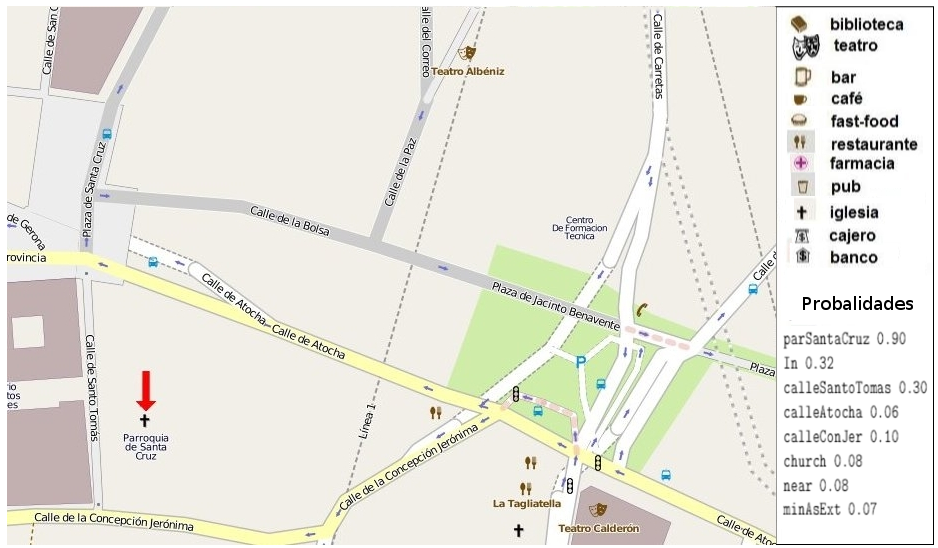
\includegraphics[width=\textwidth]{images/corpus/mapa16-prob.png}
\caption{Imagen del corpus ZOOM con target singular. Este mapa muestra un fragmento del la zona de el mapa de la Figura \ref{mapa-zoom1} pero con mayor nivel de zoom. Se muestran probabilidades de uso de las palabras en la esquina inferior derecha.}
\label{mapa-zoom2x}
\end{figure}
El mapa que analizaremos en esta secci\'on es el que se muestra en la Figura \ref{mapa-zoom2x}. Este mapa tiene un mayor nivel de zoom que el de la Figura \ref{mapa-zoom1}, y por lo tanto muestra una porci\'on m\'as peque\~na de la zona. Es decir por un lado, se ven menos objetos, pero por otro lado, lo que se v\'e tiene en general m\'as detalle, por ejemplo, se v\'e el nombre de la iglesia:
 ``Parroquia de Santa Cruz'' que no se ve\'ia en la Figura \ref{mapa-zoom1}. Otra cosa 
que se puede ver en el mapa con zoom es el nombre de la calle: ``calle de la Concepci\'on Jer\'onima'' que est\'a a la derecha de la Parroquia.
En este mapa no se puede ver el nombre del Ministerio de Asuntos Exteriores porque queda cortado en la imagen, el mismo s\'i se ve\'ia en el mapa de la Figura \ref{mapa-zoom1}. Lo \'unico que se v\'e en la calle de Santo Tom\'as es la iglesia target. Estas diferencias se van a ver reflejadas en el modelo que toma como input el algoritmo.
En la Tabla \ref{freq-mapa-zoom2x} se muestran las 12 ERs distintas dadas por los participantes que completaron el experimento en la recolecci\'on del corpus, y la cantidad de ocurrencias en el corpus. El porcentaje que representa, y si es subespecificada (SubE) o sobreespecificada (SobreE). Como dijimos anteriormente las que no son ni subespecificadas ni sobreespecificadas son minimales. Las ERs mostradas suman un total de 72, el corpus contaba con 80 ERs para esa imagen, pero 8 fueron descartadas por estar mal formadas, o no ser verdaderas para el target.
En la Tabla \ref{freq-mapa-zoom2x} se puede ver que 44 de 80 ERs son {\it Parroquia de Santa Cruz}. De las 12 ERs diferentes dadas por los las personas, 9 contienen ``Parroquia de Santa Cruz'', y acumulan un total de 69 ERs de 80. Las 3 restantes son: {\it Iglesia} con frecuencia 1 de 80, la cual era mucho m\'as frecuente para el mapa sin zoom. En este caso como en el mapa sin zoom, tambi\'en es subespecificada. {\it Iglesia cerca del Ministerio de Asuntos Exteriores}, la cual se di\'o 1 vez en el mapa con zoom, es decir tambi\'en era m\'as frecuente en el mapa sin zoom y {\it En calle de Santo Tom\'as} la cual se di\'o s\'olo 1 vez en el mapa con zoom, tambi\'en mucho m\'as frecuente en el mapa sin zoom. Esta \'ultima es una ER que identifica al target por ser el \'unico objeto que aparece en esa calle.

\begin{table}[H]
{\footnotesize
\begin{center}
\begin{tabular}{|l|l|c|c|c|c|}
\hline
&ER 					      & Cantidad &  Frecuencia & SubE&SobreE \\ \hline \hline
1&Parroquia de Santa Cruz        												 &		44&	61.1\%  &  & \\ \hline
2&Parroquia de Santa Cruz en calle de Santo Tom\'as        &    9 &	12.5\%	& &X\\ \hline
3&Parroquia de Santa Cruz en calle de Santo Tom\'as y      &    4 &     5.6\%      & &X\\
&De La Concepci\'on Jer\'onima                             &      &             & & \\ \hline
4&Parroquia de Santa Cruz en calle de Santo Tom\'as        &    3 &     4.2\%      &&X\\
&cerca de Ministerio de Asuntos Exteriores                 &      &             & &\\  \hline
5&Parroquia de Santa Cruz en calle de Santo Tom\'as        &	3 &	4.2\%	& &X\\
&entre calle de Atocha y de La Concepci\'on Jer\'onima     &	  &			&  &\\  \hline
6&Iglesia de la Parroquia de Santa Cruz			   &	2 &	2.8\%	&&X\\  \hline
7&Iglesia de la Parroquia de Santa Cruz	en      	   &	2 &	2.8\%	&&X\\  
&calle de Santo Tom\'as													 				 &		 &	    &  & \\ \hline
8&Iglesia cerca del Ministerio de Asuntos Exteriores       &	1 &	1.4	&&\\  \hline
9&En calle de Santo Tom\'as                                   &    1 &     1.4\%      &X&\\  \hline

10&Parroquia de Santa Cruz  				   &    1 &	1.4\%	&&X\\  
&cerca de Ministerio de Asuntos Exteriores		   &	  &		&&\\  \hline
11&Parroquia de Santa Cruz en calle de Atocha  		   &	1 &	1.4\%	&&X\\  
&cerca de Ministerio de Asuntos Exteriores		   &	  &		&&\\  \hline
12&Iglesia						   &    1 &	1.4\%	&X&\\  \hline
%NO ERA ER				   		   &	8 &	\%	& &\\  \hline
%\hline
\end{tabular}
\caption{ERs del corpus dadas por las personas para el mapa de la Figura \ref{mapa-zoom2x}.}\label{freq-mapa-zoom2x}
\end{center}
}
\end{table}

%\begin{table}[H]
%\begin{small}
%\begin{center}
%\begin{tabular}{|l|}
%\hline
%Palabra                                             Probabilidad\\ \hline \hline
%\textbf{\texttt{ParSantaCruz 0.90}}\\
%\textbf{\texttt{in 23/73=0.32}}\\
%\textbf{\texttt{CalleSantoTomas 0.30}}\\
%\textbf{\texttt{CalleAtocha 0.06}}\\
%\textbf{\texttt{CalleConJer 0.10}}\\
%\textbf{\texttt{church 0.08}}\\
%\textbf{\texttt{near 0.08}}\\
%\textbf{\texttt{MinisterioDeRelacionesExteriores 0.07}}\\
%\hline
%\end{tabular}
%\caption{Probabilidad de las palabras del dominio.}\label{prob-vocabulario-zoom}
%\end{center}
%\end{small}
%\end{table}

Algunas personas incluyeron en la descripci\'on al ``Ministerio de Asuntos Exteriores'' (exactamente 6 personas), siendo que el nombre del Ministerio no se v\'e en el mapa, la explicaci\'on que damos a esto es que la personas vieron el mapa sin zoom antes de ver este mapa. Como explicamos en la Secci\'on \ref{corpus-metodo} los mapas se dieron de manera aleatoria, esa aleatoriedad hizo que algunas personas recuerden lo que vieron en otros mapas. Esto es una caracter\'istica de la metodolog\'ia de recolecci\'on del corpus, que hace que las personas digan cosas que no est\'an en el modelo. 
El vocabulario y las probabilidades de uso sacadas del corpus, para el mapa de la Figura \ref{mapa-zoom2x} se ven en el mismo mapa, en la esquina inferior derecha. As\'i como en el mapa sin zoom, las probabilidades no eran parte del mapa que se mostr\'o a los participantes que completaron las ERs del corpus.

En el modelo de la Figura \ref{modelo-mapa-zoom2x} (con zoom) se ven varias diferencias con respecto al modelo de la Figura \ref{mapa-zoom1} 
(sin zoom) y esto se debe a que al acercar el zoom del mapa, algunas cosas aparecen y otras desaparecen. Se v\'e que la iglesia target no est\'a
 en la calle de Atocha como parec\'ia en el mapa mostrado en la Figura \ref{mapa-zoom1}. Se agrega el nombre de la calle de La Concepci\'on 
Jer\'onima que no se ve\'ia en el mapa anterior. Como ya mencionamos, no se v\'e el nombre del Ministerio de Asuntos Exteriores. Se agrega el nombre {\it Parroquia de Santa Cruz} que no se ve\'ia en el otro mapa. Aparece una nueva calle que est\'a en la parte superior de la manzana de la iglesia, 
de la cual no sabemos el nombre, pero le asignamos el identificador {\it str25}. Aparece el nombre de la {\it calle de Carretas}, 
cuyo identificador
 es {\it str15} en la que est\'a el restaurant {\it Medina Mayrit}, pero desaparece el nombre del restaurante. 
El edificio con identificador {\texttt d}, en este mapa se v\'e que es un teatro, el {\it Teatro Calder\'on}, tambi\'en aparece en el mapa el restaurante {\it La Tagliatela} al lado
 de un restaurante sin nombre, uno de esos restaurantes se pod\'ia ver en el mapa sin zoom. Vamos a suponer que el que se pod\'ia ver en el mapa sin zoom era {\it La Tagliatela}. Notar que dejamos de ver el nombre de la calle 
en la cual se ubica el teatro y los restaurantes reci\'en nombrados.


\begin{figure}[H]
\centering
\begin{tikzpicture}
  [
    n/.style={circle,draw,inner sep=3pt,node distance=4cm},
    aArrow/.style={->, >=stealth, thick, shorten <= 1pt, shorten >= 1pt},	
  ]
	\node[n,label=below:{
    \relsize{-2}$\begin{array}{c}
     \nStreet\end{array}$}] (a) {\relsize{-2}$str17$};		
	 \node[n,label=above:{
    \relsize{-2}$\begin{array}{c}
      \nBuilding\end{array}$}, above of=a] (f) {\relsize{-2}$min1$};	
					 
	\node[n,label=above:{
    \relsize{-2}$\begin{array}{c}
		 \nChurch\\[-3pt] 
     \nParroquiaDeSantaCruz\end{array}$}, above of=f] (g) {\relsize{-2}$church1$};
	\node[n,label=above:{
    \relsize{-2}$\begin{array}{c}
      \nStreet\\[-3pt] 
      \nCalleDeLaConcepcionJeronima\end{array}$}, above of=g] (z) {\relsize{-2}$str22$};
			
	\node[n,label=above:{
    \relsize{-2}$\begin{array}{c}
      \nStreet\end{array}$}, right of=z] (y) {\relsize{-2}$str25$};	
				
	\node[n,label=below:{
    \relsize{-2}$\begin{array}{c}
      \nStreet\\[-3pt] 
      \nCalleDeElSalvador\end{array}$}, right of=a] (b) {\relsize{-2}$str12$};
   
	\node[n,label=below:{
    \relsize{-2}$\begin{array}{c}
      \nStreet\end{array}$}, right of=b] (m) {\relsize{-2}$str16$};		 

  \node[n,label=above:{
    \relsize{-2}$\begin{array}{c}
      \nStreet\\[-3pt] 
      \nCalleSantoTomas\end{array}$}, above of=b] (c) {\relsize{-2}$str10$};	
			
  \node[n,label=below:{
    \relsize{-2}$\begin{array}{c}
     \nChurch\end{array}$}, right of=c] (d) {\relsize{-2}$church2$};
			
  \node[n,label=above:{
    \relsize{-2}$\begin{array}{c}
      \nRestaurante\end{array}$}, above of=d] (h) {\relsize{-2}$rest3$};			
			
  \node[n,label=above:{
    \relsize{-2}$\begin{array}{c}
      \nStreet\\[-3pt] 
      \nCalleAtocha\end{array}$}, above of=c] (e) {\relsize{-2}$str9$};		

  \node[n,label=right:{
    \relsize{-2}$\begin{array}{c}
      \nRestaurante\\[-3pt] 
      \nLaTagliatella\end{array}$}, right of=m] (k) {\relsize{-2}$rest4$};

 \node[n,label=below:{
    \relsize{-2}$\begin{array}{c}
      \nRestaurante\end{array}$}, below of=k] (w) {\relsize{-2}$rest5$};

  \node[n,label=below:{
    \relsize{-2}$\begin{array}{c}
      \nTeatroCalderon\end{array}$}, right of=d] (i) {\relsize{-2}$thea0$};
		
  \node[n,label=above:{
    \relsize{-2}$\begin{array}{c}
      \nStreet\\[-3pt] 
      \nCalleDeCarretas\end{array}$}, right of=h] (x) {\relsize{-2}$str15$};	

%\node[n,label=below:$str17\nStreet$,label=above:{
 %   \relsize{-2}}, below of=k] (n) {};				
 \draw [aArrow,<->,bend right=40] (g) to node[auto,swap]{\relsize{-2}$\nFrenteCerca$} (f);
% \draw [aArrow,bend right=40] (f) to node[auto,swap]{\relsize{-2}$\nFrenteCerca$} (g);

 \draw [aArrow,bend right=40] (g) to node[auto,swap]{\relsize{-2}$\nIn$} (c);
 \draw [aArrow,bend right=20] (g) to node[auto,swap]{\relsize{-2}$\nIn$} (z);
 \draw [aArrow,bend right=20] (g) to node[auto,swap]{\relsize{-2}$\nIn$} (y);
 \draw [aArrow,bend right=40] (d) to node[auto,swap]{\relsize{-2}$\nIn$} (m);
 \draw [aArrow,<->,bend right=-20] (d) to node[auto,swap]{\relsize{-2}$\nFrenteCerca$} (i);
 %\draw [aArrow,bend right=40] (i) to node[auto,swap]{\relsize{-2}$\nFrente$} (d);
 \draw [aArrow,<->,bend right=-20] (k) to node[auto,swap]{\relsize{-2}$\nCerca$} (d);
 \draw [aArrow,<->,bend right=40] (k) to node[auto,swap]{\relsize{-2}$\nCerca$} (w);
 %\draw [aArrow,bend right=40] (d) to node[auto,swap]{\relsize{-2}$\nCerca$} (k);
 \draw [aArrow,<->,bend right=40] (k) to node[auto,swap]{\relsize{-2}$\nIn$} (x);
 \draw [aArrow,bend right=40] (k) to node[auto,swap]{\relsize{-2}$\nIn$} (m);
 \draw [aArrow,<->,bend right=40] (k) to node[auto,swap]{\relsize{-2}$\nFrenteCerca$} (i);
% \draw [aArrow,bend right=40] (i) to node[auto,swap]{\relsize{-2}$\nFrente$} (k);
 \draw [aArrow,bend right=20] (h) to node[auto,swap]{\relsize{-2}$\nIn$} (e);
 \draw [aArrow,bend right=20] (h) to node[auto,swap]{\relsize{-2}$\nIn$} (j);

 \draw [aArrow,bend right=30] (f) to node[auto,swap]{\relsize{-2}$\nIn$} (c);
 \draw [aArrow,bend right=40] (f) to node[auto,swap]{\relsize{-2}$\nIn$} (e);
 \draw [aArrow,bend right=40] (f) to node[auto,swap]{\relsize{-2}$\nIn$} (a);
 \draw [aArrow,bend right=40] (f) to node[auto,swap]{\relsize{-2}$\nIn$} (b); 

 \draw [aArrow,bend right=5] (i) to node[auto,swap]{\relsize{-2}$\nIn$} (e);
 \draw [aArrow,bend right=40] (i) to node[auto,swap]{\relsize{-2}$\nIn$} (m);

 \end{tikzpicture}
\caption{Modelo relacional del mapa de la Figura \ref{mapa-zoom2x}.}
\label{modelo-mapa-zoom2x}
\end{figure}


Se ejecut\'o el algoritmo 1000 veces con las probabilidades de uso que se muestran en la esquina inferior derecha del mapa de la Figura \ref{mapa-zoom2x}, con el modelo que se muestra en la Figura \ref{modelo-mapa-zoom2x} y las ERs obtenidas se muestran en la Tabla \ref{formulas-mapa-zoom2x}.

%Como dijimos $\exists \nIn(T)$ quiere decir que est\'a en una calle, se puede ver en la 2da f\'ormula, as\'i mismo $\exists.\nCerca$ quiere decir que tiene algo cerca, en este caso es el Ministerio de Asuntos Exteriores.

Como resultados podemos ver que el algoritmo gener\'o {\it Parroquia de Santa Cruz} en 57\% de las ejecuciones, y esto es muy cercano al porcentaje que fue generada por las personas en el corpus (61.1\%). La segunda ER m\'as generada por las personas tambi\'en est\'a en 3ra posici\'on del top 10 ranking del algoritmo con una frecuencia del 7.2\%, las personas la generaron un 12.5\%. La 3ra, 4ta, 5ta, 7ma, 11ava ERs m\'as dadas por las personas en el corpus, son sobreespecificadas y consideramos que justamente por eso el algoritmo no las gener\'o, la sobreespecificaci\'on que permite el algoritmo es limitada, entonces, no agrega tanta informaci\'on redundante. La 6ta ER fue generada por las personas en un 2.78\% y por el algoritmo en 4.8\%. Recordemos el {\it Ministerio de Asuntos Exteriores} no pertenec\'ia al modelo, por lo tanto, el algoritmo no pod\'ia generar las ERs que lo incluyeran.% {\it Iglesia cerca del Ministerio de Asuntos Exteriores} y 

%\begin{table}[H]
%\begin{center}
%\begin{tabular}{|l|l|c|}
%\hline
%&F\'ormula			      &  \# \\ \hline \hline
%1& $\exists \nParroquiaDeSantaCruz$& 570\\ \hline

%2& $\exists \nParroquiaDeSantaCruz. \exists \nIn(T)$& 174\\ \hline
%3& $\exists \nParroquiaDeSantaCruz. \exists \nIn(\exists \nCalleSantoTomas)$& 72\\ \hline
%4& $\exists \nParroquiaDeSantaCruz. \land \exists.\nCerca(T)$& 57\\ \hline

%5& $\exists \nChurch \land \exists \nParroquiaDeSantaCruz$& 48\\ \hline
%6& $\exists \nChurch \land \exists \nParroquiaDeSantaCruz. \exists \nIn(T)$& 17\\ \hline
%7& $\exists \nParroquiaDeSantaCruz \land \exists. \nIn(\exists \nCalleConJer)$& 13\\ \hline
%8& $\exists \nChurch \land \land \exists. \nIn(\exists \nCalleConJer) $&10\\ \hline

%9& $\exists \nIn(\exists \nCalleSantoTomas) \land \exists \nChurch$&9\\ \hline

%10& $\exists \nChurch \land \exists \nIn(\exists \nCalleSantoTomas))$&7\\ \hline

%\end{tabular}

%\caption{Las 11 f\'ormulas dadas por el algoritmo para el modelo de la Figura \protect\ref{modelo-mapa-zoom2x}.}\label{formulas-mapa-zoom2x}
%\end{center}
%\end{table}
\begin{table}[H]
\begin{center}
\begin{tabular}{|l|l|c|c|}
\hline
&ER			      &  \# &\% \\ \hline \hline
1& Parroquia de Santa Cruz& 801&80.1\\ \hline
%2& & \\ \hline
2& Parroquia de Santa Cruz en Calle de Santo Tom\'as& 72&7.2\\ \hline
%4& & \\ \hline
3& Iglesia de la Parroquia de Santa Cruz& 65&6.5\\ \hline
%6& & \\ \hline
4& Iglesia en Calle de Santo Tom\'as&16&1.6\\ \hline
5& Parroquia de Santa Cruz en Calle de la Concepci\'on Jer\'onima& 13&1.3\\ \hline
6& Iglesia en Calle de la Concepci\'on Jer\'onima &10&1\\ \hline

%10& &\\ \hline

\end{tabular}

\caption{Posibles realizaciones de las f\'ormulas que di\'o el algoritmo para el modelo de la Figura \protect\ref{modelo-mapa-zoom2x}.}\label{formulas-mapa-zoom2x}
\end{center}
\end{table}

Por los resultados obtenidos vemos que las probabilidades de uso, son una buena gu\'ia para el algoritmo para conseguir un ranking de ERs que se acerca bastante al dado por las personas. Vemos que el 95\% de las ERs generadas por el algoritmo tiene {\it Parroquia de Santa Cruz}, esto es mayor a 0.90 que es la probabilidad de uso, y esto se debe a que a veces aparece sobreespecificada. Tambi\'en vemos que las calles {\it Santo Tomas} y {\it de la Concepci\'on Jer\'onima} aparecen m\'as que las calles con probabilidad de uso menor. Tambi\'en vemos que rara vez aparece una relaci\'on que tenga probabilidad de uso menor a 0.1.     


\begin{table}[H]
{\footnotesize
\begin{center}
\begin{tabular}{|l|l|c|c|}
\hline
&ERs para el target {\it church1} 					       &  Frecuencia & Frecuencia-Alg \\ \hline \hline
1&Parroquia de Santa Cruz        						   &	61.1\%  &   \\ \hline
2&Parroquia de Santa Cruz en calle de Santo Tom\'as        &    12.5\%	&   \\ \hline
3&Parroquia de Santa Cruz en calle de Santo Tom\'as y      &    5.6\%   & \\
&De La Concepci\'on Jer\'onima                             &            &  \\ \hline
4&Parroquia de Santa Cruz en calle de Santo Tom\'as        &     4.2\%  &\\
&cerca de Ministerio de Asuntos Exteriores                 &            &\\  \hline
5&Parroquia de Santa Cruz en calle de Santo Tom\'as        &	3       &	4.2\%	 \\
&entre calle de Atocha y de La Concepci\'on Jer\'onima     &	        &			 \\  \hline
6&Iglesia de la Parroquia de Santa Cruz			           &	2.8\%	&\\  \hline
7&Iglesia de la Parroquia de Santa Cruz	en      	       &	2.8\%	&\\  
&calle de Santo Tom\'as									   &	    	&	    \\ \hline
8&Iglesia cerca del Ministerio de Asuntos Exteriores       &	1.4	    &\\  \hline
9&En calle de Santo Tom\'as                                &   1.4\%    &\\  \hline

10&Parroquia de Santa Cruz  				               &    1.4\%	&\\  
&cerca de Ministerio de Asuntos Exteriores		           &	  		&\\  \hline
11&Parroquia de Santa Cruz en calle de Atocha  		       &	1.4\%	&\\  
&cerca de Ministerio de Asuntos Exteriores		   	       &	    	&\\  \hline
12&Iglesia						                           &    1.4\%	&\\  \hline
%NO ERA ER				   		   &	8 &	\%	& &\\  \hline
%\hline
\end{tabular}
\caption{Comparaci\'on de las ERs del corpus con las generadas por el algoritmo para la Figura \ref{mapa-zoom2x}.}\label{compara-mapa-zoom2x}
\end{center}
}
\end{table}



\subsection{Plural sin zoom}
\label{sec:plural}

%Como dijimos el nombre del Ministerio de Asuntos Exteriores no se ve en el mapa, sin embargo 6 personas lo usaron en sus ERs, 
%esto se debe a que como en la obtenci\'on del corpus los mapas se mostraron aleatoriamente, algunas personas vieron el mapa sin zoom antes, y recordaron que ese edificio que se v\'e en el mapa, es el Ministerio de Asuntos Exteriores. Como no est\'a visible en el mapa, no aparece en el modelo.

En esta secci\'on mostramos la GER en un mapa con target plural, sin zoom. Como podemos ver en el mapa de la Figura \ref{mapa-zoom-plural} el conjunto target est\'a compuesto por 2 restaurantes, uno que tiene nombre {\it Restaurante Medina Mayrit} y el otro est\'a ubicado cerca (a unos 100 metros), al lado de una iglesia. Estos casos son m\'as complejos ya que por ejemplo, el restaurante que no tiene nombre, no est\'a ubicado en la {\it calle de Atocha}, pero en la imagen parece cerca. El corpus de las ERs dadas por las personas contiene muchos errores de este tipo, las ERs se muestran en la Tabla \ref{freq-mapa-zoom-plural} se muestran las ER, la cantidad de ocurrencia en el corpus, si es Parcial y si es sobreespecificada (SobreE). 
Recordemos que en el Cap\'itulo \ref{sec:seleccion} dimos la definici\'on de ER parcial, y es aquella que siendo plural, identifica a un conjunto inclu\'ido estrictamente en el target.


\begin{figure}[H]
\centering
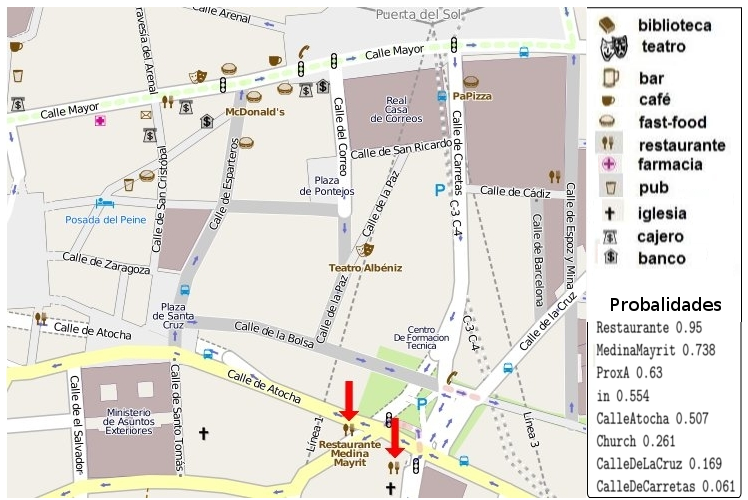
\includegraphics[width=\textwidth]{images/corpus/mapa10conProb.png}\\[0pt]
\caption{Imagen sin zoom, target plural. Las probabilidades de uso de las palabras se muestran en la esquina inferior derecha.}
\label{mapa-zoom-plural}
\end{figure}

De las ERs que se ven en la tabla 55\% son parciales, 25\% son sobreespecificadas. Cabe notar que el algoritmo no va a generar ERs parciales, ni ERs que nombran cosas que no son ciertas para el target... como por ejemplo para el restaurante que no tiene nombre no est\'a en la {\it calle de Atocha}, por lo tanto no est\'a en la {\it calle de Atocha} en el modelo, y el algoritmo no podr\'a generarlas. Al no generar ERs parciales el algoritmo no podr\'a generar las ERs 1, 6, 7, 9, 10, 12, 13 ,14, 15 y 17. De las restantes no podr\'a generar 12, 14, y 15 por decir que el restaurante sin nombre est\'a en la {\it calle de atocha}. Por lo tanto quedan 7 ERs distintas que el algoritmo deber\'ia ser capaz de generar 1, 6, 7, 9, 10, 13 y 15. %El conjunto de ERs que el algoritmo puede generar es el 32.67\% del corpus para la imagen considerada, que teniendo en cuenta que tiene s\'olo 60 ERs 

Ejecutamos el algoritmo 1000 veces, con input el modelo que se mostr\'o en la Figura \ref{modelo-mapa-zoom}, las probabilidades de uso de las palabras calculadas como se muestra en la Secci\'on \ref{sec:learning-corpus} del Cap\'itulo \ref{sec:algoritmo} se muestran en la esquina inferior derecha de la Figura \ref{mapa-zoom-plural}. El modelo coincide con el modelo de la Figura \ref{modelo-mapa-zoom}, ya que es el mismo mapa.


\begin{table}[H]
{\footnotesize
\begin{center}
\begin{tabular}{|l|l|c|c|c|c|}
\hline
&ER 					      & Cantidad &  \% & Parcial & SobreE\\ \hline \hline
1&Medina Mayrit y el que esta cerca        &	11	&	18.33\% &  &  \\ \hline


2&Medina Mayrit			&11		&	18.33\%	&X&\\  \hline


3&Restaurantes de calle de Atocha				&	8  &	13.33\%	&X&\\ \hline

4&Medina Mayrit y el que est\'a en calle de Atocha	      &5		&	8.33\%	&&\\ \hline

5&el de la calle Atocha y De La Cruz       &	3  &	5\%	&X & \\  \hline
6&Medina Mayrit y el que est\'a cerca				&		3 &	5\%  & &X\\
&cercano a la iglesia				&	  &	&&\\ \hline
7&Medina Mayrit en calle de Atocha y el que est\'a cerca				& 3  &	5\%	&&X\\
&cerca de la iglesia				&	  &		&&\\ \hline

8&calle de Atocha				&	2  &	3.33\%	&X&\\ \hline

9&Medina Mayrit y el que est\'a cerca			&2  &	3.33\%	&&X\\
&en calle de La Cruz	&	  &		&&\\ \hline

10&Medina Mayrit y el que est\'a 	&	2	&	3.33\%  &&X\\
&cerca de la iglesia				&	  &	&&\\ \hline
11&El que est\'a en calle de Atocha y Carretas 					&	2  &	3.33\%	&X&\\ \hline
12&Medina Mayrit y el que est\'a cerca				&	2	&	3.33\%  &&X\\
&en la calle Atocha y De La Cruz        &	  &	&&\\ \hline
13&Medina Mayrit en calle de Atocha y el que est\'a cerca			&1  &	1.67\%	&&X\\
&en calle de La Cruz	&	  &		&&\\ \hline

14&Medina Mayrit y el que est\'a cerca			&1  &	1.67\%	&&X\\
&en calle de Atocha	&	 &		&&\\ \hline

15&El que esta en calle de Atocha y Carretas, 	      &	1	&	1.67\%	&&\\
&y el de Atocha y de la Cruz	      &		&	&&\\ \hline


16&pr\'oximo a la iglesia 	      &1		&	1.67\%	&X &\\ \hline

17&Medina Mayrit en calle de Atocha y el que est\'a cerca  				&  1 &	1.67\%	&&X\\ \hline
&calle de Atocha y calle de La Cruz  					&1  &	1.68\%	&X&\\ \hline 
\hline
Totales	&&60	&	100\%	&&\\

\hline
\end{tabular}
\caption{ERs del corpus dadas por humanos para el mapa de la Figura \ref{mapa-zoom-plural}.}\label{freq-mapa-zoom-plural}
\end{center}
}
\end{table}

En el ap\'endice \ref{formulas-plurales}, se muestran las f\'ormulas generadas por el algoritmo.


\begin{enumerate}
\item 
\end{enumerate}    

En la Tabla \ref{formulas-mapa-zoom2} podemos ver que la ER con mayor frecuencia que gener\'o el algoritmo es parecida a la de mayor frecuencia en el corpus, la realizaci\'on podr\'ia ser {\it El restaurante Medina Mayrit y el que est\'a cerca del restaurante Medina Mayrit}, siendo que la que dijeron las personas en el corpus con m\'as frecuencia fue {\it El restaurante Medina Mayrit y el que est\'a cerca}, alguien podr\'ia decir que le falta un objeto, {\it est\'a cerca} de qu\'e?, y s\'i se refiere al mismo restaurante. Estas cosas son dif\'iciles de generar autom\'aticamente. Como mencionamos antes, vemos que hay f\'ormulas que tienen $\exists \nCerca.(\exists \nCerca.(\exists \nMedinaMayrit))$ que denota al mismo objeto. Preveemos sacar estas cosas en trabajo futuro, vea el Cap\'itulo \ref{sec:conclusiones}. Otra cosa ya vista en los otros mapas, es la tautolog\'a $\exists \nIn.(T)$, que es decir que est\'a en una calle, tambi\'en ser\'a estudiada en trabajo futuro.


\section{Notas finales y linkeo del cap\'itulo}
%%%%%%%%%%%%%%%%%%%%%%%%%%%%%%%%%%%%%%%%%%%%%%%%%%%%%%%%%%%%%%%%%%%%%%%%%%%%%%%%%%%%%%%%%%%%%%%%%%%%%%%%%%%%%%%%%%%%%%%%%%%%%%%%%%%%%%%%%%%%%%%%%%%%%%%%%%	       >2
\label{sec-final}

En este cap\'itulo vimos como se recolect\'o el corpus Zoom, los materiales que se usaron para la recolecci\'on estan en Ap\'endice \ref{corpus-apendice}, la anotaci\'on del corpus, el an\'alisis y evaluaci\'on del mismo. 
Este corpus se cre\'o viendo la necesidad de existencia de recursos en dominios m\'as naturales. Se recolect\'o mediante un experimento on-line en el que las personas ve\'ian un mapa el cual conten\'ia una o dos flechas indicando el o los targets y completaban una ER dirigida a un amigo en la cual ten\'ian que describir el o los objetos sen\~alados. Cada persona di\'o 20 ER 10 singulares y 10 plurales, de esas 10 singulares o plurales, hab\'ia 5 con alto nivel de zoom y 5 con bajo nivel de zoom.
El corpus tiene en cuenta un dominio que es significativamente m\'as cerca de aplicaciones del mundo real, y aborda las situaciones m\'as complejas de referencia de los recursos existentes de este tipo nombrados en el Cap\'itulo \ref{sec:corpus2}. En particular, el dominio de zoom hace uso de contextos con diferentes niveles de detalle, y contiene ejemplos de referencia singular y plural producido por un n\'umero relativamente grande de hablantes en ambos idiomas espa\~nol y portugu\'es, siendo el lenguaje seleccionado el lenguaje nativo de la persona.
En este corpus podemos encontrar distintos tipos de ER como las nombradas en el Cap\'itulo \ref{sec:seleccion}, tenemos varias ER por mapa con lo cual podremos luego calcular las probabilidades de uso de las palabras como se explic\'o en \ref{sec:learning} para ejecutar nuestro algoritmo explicado en el Cap\'itulo \ref{sec:algoritmo}. Dadas las caracter\'isticas de los mapas usados para la recolecci\'on, el corpus tiene ER relacionales, proposicionales, de plurales, sobre-especificadas y hasta under-especificadas.
El corpus fue anotado por 2 personas y finalmente un juez decidi\'io cual anotaci\'on dejar, la anotaci\'on se hizo teniendo en cuenta atributos para el target tipo, nombre, en (refiri\'endose a donde est\'a, en que calle), relaciones espaciales (izquierda, derecha, en esquina / entre, cerca, en-frente-de, detr\'as) estas relaciones requer\'ian la ER de otros objetos (landmarks), en algunos caso solo uno, y en otros 2, y el \'ultimo atributo disponible fue {\it otro}, para anotar cosas que no se hab\'ian tenido en cuenta en la anotaci\'on nombrada. Para cada uno de los landmarks se tuvieron en cuenta 4 atributos m\'as, con lo que para cada ER tenemos un m\'aximo de 26 atributos o relaciones cuando el target era singular y 52 cuando el target era plural. El atributo {\it otro} nos ayuda en el sentido de que podemos agrupar las ER que solo difieren en este atributo, pero nos juega en contra ya que esas ER que contienen {\it otro} no las podremos generar, es decir perdemos parte de la informaci\'on que la persona di\'o. Se midi\'o el porcentaje de acuerdo (kappa) entre los jueces y fue del 84\%. 
Se realiz\'o una evaluaci\'on cuyos resultados preliminares de un enfoque basado en SVM a GER - que fueron \'unicamente presentados para la futura evaluaci\'on de algoritmos GER basados en datos Zoom - alusi\'on a la complejidad real de la tarea GER en este dominio.
En primer lugar, nos damos cuenta de que un enfoque basado en SVM similar en~\cite{thiago-svm} en datos de GRE3D3 y GRE3D7 ha obtenido considerablemente mayor exactitud media (0,46 y 0,64 respectivamente) y una mayor media de las puntuaciones de Dice (0,78 y 0,89 respectivamente). Esto, por supuesto, se explica por el aumento de la complejidad del dominio Zoom (por ejemplo, en el n\'umero de posibles objetos y propiedades at\'omicas y relacionales etc.). 
Sin embargo, nos damos cuenta tambi\'en que el esquema de anotaci\'on Zoom  aunque teniendo en cuenta ya gran n\'umero de posibles atributos - sigue siendo demasiado simple. En particular, el atributo {\em otro} ha sido usado en exceso y, como consecuencia, las posibilidades de reproducci\'on de las descripciones corpus es pequen\~a. Es evidente que a\'un queda trabajo por hacer para ampliar el esquema de anotaci\'on y dividir lo que se anot\'o como {\em otros} en un mayor n\'umero de atributos.
En segundo lugar, las descripciones de zoom son propensas a transmitir las relaciones entre un solo objeto y varios objetos emblem\'aticos, como en `el restaurante en la calle 5, cerca de la biblioteca '. Aunque es com\'un en el uso del lenguaje, el uso de m\'ultiples propiedades relacionales de esta manera ha sido poco investigado, tal vez debido a que puede dar lugar a descripciones ambiguas, como en `el restaurante cerca de la iglesia en la calle Jackson y el bar en la calle 5' para un restaurante situado cerca del cruce de estas dos calles.
Como trabajo futuro, tenemos la intenci\'on de hacer que el corpus quede a disposici\'on p\'ublica para la investigaci\'on sobre m\'ultiples aspectos de la selecci\'on de contenidos y la realizaci\'on de superficie en GER. En particular, prevemos el uso del corpus zoom como datos de entrenamiento y prueba de modelos de aprendizaje autom\'atico de GER, y tambi\'en para abordar otras cuestiones que no se han abordado en el presente trabajo. Estos incluyen la generaci\'on de expresiones referenciales de bases de conocimiento con diferentes grados de detalle aprovechando que el corpus tiene esa caracter\'istica, y las cuestiones de la variaci\'on entre los hablantes y del mismo hablante en GER.
Se realiz\'o un caso de estudio para 3 mapas del ZOOM corpus, y se vi\'o que el algoritmo es capaz de conseguir ERs que se encuentran en corpora, y a\'un m\'as cuando tenemos entornos con target plural, el algoritmo siempre d\'a una ER, teniendo una ventaja significativa con respecto a las personas, las cuales dieron en m\'as del 50\% ERs parciales o que conten\'ian cosas que no eran ciertas en la imagen considerada. A pesar de las ventajas del algoritmo vemos que hay cosas que todav\'ia quedan por pulir como ser tautolog\'ias encontradas en las f\'ormulas, o propiedades circulares que se podr\'ian sacar, o directamente no permitir.
%\section{Conclusiones y linkeo del cap\'itulo}

 

